% Copyright (c) 2021 Tobias Briones. All rights reserved.
% SPDX-License-Identifier: CC-BY-4.0
%
% This file is part of https://github.com/tobiasbriones/
% cp-unah-mm700-agricultural-soil-sampling-for-data-analysis
%
% This source code is licensed under the Creative Commons Attribution 4.0
% International License found in the LICENSE-CC file in the root directory of
% this source tree or at https://spdx.org/licenses/CC-BY-4.0

\documentclass[conference]{IEEEtran}
\usepackage{article}

\title{
MODELO DE MUESTREO VIRTUAL DE SUELOS AGRÍCOLAS EN HONDURAS PARA ANALÍTICA EN BASE AL MUESTREO ALEATORIO SIMPLE Y ESTRATIFICADO
}

\author{
\IEEEauthorblockN{Tobias Briones}
\IEEEauthorblockA{\textit{Universidad Nacional Autónoma de Honduras} \\
\textit{Carrera de Licenciatura en Matemática}\\
San Pedro Sula, Honduras \\
tobias.briones@unah.hn} \\\vspace*{20pt} \normalsize
Diciembre 2021
}
\date{Septiembre 2021}

% ----- THIS DOCUMENT CONTAINS ALL THE BLUEPRINT PIECES TOGETHER -----

\begin{document}

\maketitle

\begin{center}
    
\includegraphics[width=0.3\linewidth]{ref/logo-unah.png}\\[4ex]
    \textit{Universidad Nacional Autónoma de Honduras}

    \bigbreak

    \textit{Proyecto de Seminario de Investigación Presentado a la Carrera de Licenciatura en Matemática}
\end{center}

\begin{abstract}
El desarrollo de soluciones de ciencia de datos para agricultura en Honduras comprende varias dificultades, a saber, los recursos de cómputo disponibles en los entornos de producción, la educación tecnológica y de toma de decisiones de los usuarios interesados y el contexto específico para poder realizar un análisis de sistemas. Esta investigación provee un modelo de muestreo virtual para el analista de datos de forma que sea posible desplegar conjuntos de datos históricos muestreados para optimizar los modelos de análisis de datos que los consumen y que se actualizan periódicamente. El resultado es un artefacto mínimo viable de investigación consistente en una API que permite utilizar modelos, visualización geográfica, reportes y resultados con un conjunto de datos propiamente muestreados mediante un muestreo aleatorio simple estratificado. Así también, se provee un marco teórico para que en conjunto, tanto el analista como la empresa agrícola converjan a una apropiada obtención de datos y puedan eventualmente ejecutar toma de decisiones informadas. Por último, estos resultados impulsan la educación tecnológica y la implementación de ciencia de datos y sistemas de información en las empresas siendo estas características en primera clase de países desarrollados.
\end{abstract}

\bigbreak

\begin{abstract}
The development of data science solutions for agriculture in Honduras involves several difficulties, namely, the computing resources available in the production environments, the technological education and decision-making of stakeholders and the specific context to be able to carry out a system analysis. This research provides a virtual sampling model for the data analyst so that it is possible to deploy sampled historical datasets to optimize the data analysis models consuming them and that are periodically updated. The result is a minimum viable research artifact consisting of an API that allows the use of models, geographic visualizations, reports, and results with a dataset properly sampled through the stratified simple random sampling. Likewise, a theoretical framework is provided so that together, both the analyst and the agricultural company converge to an appropriate data collection and can eventually execute informed decision-making. Finally, these results drive technological education and the implementation of data science and information systems into companies, which are first class characteristics of developed countries.
\end{abstract}

\bigbreak

\begin{IEEEkeywords}
sampling, analytics, agricultural-modeling, honduras, data-science
\end{IEEEkeywords}

% ------------------------------  INTRODUCTION  ------------------------------ %


\section{Introducción}

En la ciencia de datos \footnote{La ciencia de datos combina múltiples campos, como las estadísticas, los métodos científicos, la inteligencia artificial (IA) y el análisis de datos para extraer el valor de los datos \cite{oracle-data-science-2021}.} se desarrollan procesos complicados para obtener valor a partir de los datos crudos de los usuarios de forma que se puedan entrenar modelos para hacer predicciones, prescripciones e investigación de los problemas de las empresas en una base de caso por caso. Uno de los primeros pasos en el proceso consiste en obtener datos existentes y que sufran una transformación para que se filtren o curen y por tanto se obtengan datos relevantes al estudio. Así también como determinar la clasificación correcta de los datos, determinar variables de estudio, desnormalizar bases de datos, encontrar patrones y establecer  interpretaciones \cite{university-of-wisconsin-data-science-2021}. Debido a estos retos técnicos, el analista de datos \footnote{El analista de datos actúa como guardián de los datos de una organización para que las partes interesadas puedan comprender los datos y usarlos para tomar decisiones comerciales estratégicas \cite{eastwood-data-analyst-2021}.} debe de contar como entrada con todos los datos e historiales de la empresa que se va a analizar en ese dominio.

\bigbreak

A fin de obtener los datos de fincas, granjas o terreno agrícola es requerido muchas veces realizar muestreo de suelo. Algunos de los casos de uso son diagnóstico de fertilidad \cite{lassaga-2011} y análisis de contaminantes \cite{gobpe-ministerio-del-ambiente-2014}. Es determinante construir resultados a partir de estos datos para dar resultados en base a zafra y sus correspondiente diagnóstico de optimalidad con respecto a rendimiento.

\bigbreak

Existen varios enfoques de muestreo de una población, la mayor parte de las veces se basan en un muestreo aleatorio simple. Para poder diseñar un muestreo para un caso en particular es requerido llevar a cabo encuestas puntuales al personal del área agrícola a fin de conocer el terreno y sus clasificaciones \cite{organizacion-de-las-naciones-unidas-para-la-agricultura-y-la-alimentacion-1990}.

\bigbreak

Para realizar un diseño de muestreo es necesario indagar en la teoría de muestreo elemental, recurrir a la ciencia de datos en las primeras etapas del análisis de estos casos de uso (transformaciones de datos que se obtienen al inicio del proceso de analítica) y definitivamente a las herramientas que llevarán a cabo el artefacto de investigación consistentes en las bibliotecas de ciencia de datos de Python \footnote{Python es un lenguaje de programación de propósito general de alto nivel e interpretado \cite{wikipedia-python-2021}.} \cite{grus-2015} \cite{geopandas-developers-2021}. Por último, sin dejar de lado el otro aspecto complementario para diseñar tal muestreo, se deberá tener en consideración algunas condicionantes del área local en Honduras de forma que el artefacto de investigación sea desplegable en los casos de uso que conciernen más a esta área geográfica \cite{fao-2004}.

\subsection{Justificación}

El propósito de esta investigación es diseñar un proceso eficiente que permita modelar los suelos agrícolas de forma que se puedan obtener muestras representativas de estos y posteriormente ser utilizables para que permitan desarrollar proyectos con el sector agrícola integrando los resultados obtenidos de esta investigación. Se ha propuesto como objetivo emprender una investigación en este campo relacionado con el análisis de los suelos agrícolas para poder integrar los modelos obtenidos en proyectos de analítica. Esto se espera que permita a las empresas de analítica \footnote{La analítica reúne la teoría y la práctica para identificar y comunicar conocimientos basados en datos que permiten a los gerentes, partes interesadas y otros ejecutivos de una organización tomar decisiones más informadas \cite{eastwood-data-analyst-2021}.} poder proveer servicios/productos con un estado del arte en la región para sus prospectos clientes o usuarios los cuales consisten en empresas agrícolas en Honduras que deberían automatizar y llevar a cabo el análisis de suelos de forma más moderna que como lo hacen actualmente o, en el peor de los casos, no hacen ni son capaces de entender ningún análisis ni optimización u automatización en absoluto. Los beneficiados serán primero, empresas del sector agrícola en Honduras al poder darle uso a los históricos actuales y futuros de sus datos a fin de modelar sus suelos o lotes y así optimizar sus operaciones mediante técnicas de análisis de datos, lo cual ya se puede hacer. La diferencia es que, por el otro lado, se tiene como beneficiado segundo a los proveedores de servicios de analítica al poder entrenar y desplegar los modelos de ciencia de datos de forma \textit{más eficiente} si se utiliza un muestreo virtual propuesto en esta investigación. Los recursos para realizar la extracción de datos en el suelo agrícola son muy limitados ya que la población es demasiado grande. Se debe poder entrenar los respectivos modelos de analítica a partir de los datos obtenidos del muestreo el cual debe ser suficientemente representativo y pequeño para poder llevar a cabo esta extracción de datos utilizando los recursos limitados que se tienen disponibles. En síntesis, las empresas agrícolas tienen ya sus históricos, las empresas de analítica en teoría pueden optimizar en base a esos datos (muestra física) pero es aún posible tener mayor ganancia para ambos sector agrícola y sector de analítica al hacer que el análisis sea más eficiente al reducir esa entrada de datos mediante un segundo muestreo que será virtual.

\bigbreak

Según el \textit{Tratado Internacional de  Recursos Fito Genéticos  para la Alimentación y la Agricultura  TIRFAA} del \textit{Gobierno de la República de Honduras $\mid$ Secretaría de Agricultura y Ganadería} (2019) \cite{santacreo-2019} \say{En la actualidad no se cuenta con un inventario exhaustivo a nivel nacional de las variedades tradicionales cultivadas en fincas, principalmente de pequeños productores (campesinos), los parientes y especies silvestres utilizadas para la producción de alimentos}. Lo cual sugiere que es importante que los datos sobre las variedades de diversos productores en el país deberían ser explotados para tener manejo sobre el valor que puede agregar la ciencia de datos a esas brechas de inventario existentes.

\bigbreak

Como limitantes en este proyecto se encuentran: la cota de tiempo para su realización consistente en un curso trimestral de seminario de investigación. Por otra parte, llevar a cabo la recopilación física de datos o muestras no es necesario ya que el muestreo físico va por parte del sector agrícola; siendo así, una potencial limitante es poder obtener un conjunto de datos apropiado de acceso abierto para poder hacer la demostración del procedimiento en cuestión. Debido a estas limitaciones se define el alcance del proyecto abajo.

\subsection{Audiencia}

Esta investigación involucra a todos aquellos interesados en la industria de analítica/ciencia de datos y de agricultura en Honduras. El tema se define en base a la etapa intermedia entre la empresa agrícola que cuenta con datos de muestreo físico y la empresa de analítica/ciencia de datos que ha de entrenar modelos en base al propuesto muestreo virtual.

\subsection{Alcance}

Dado las limitantes de esta investigación, se procederá a realizar las siguientes metas:

\begin{itemize}
    \item Obtener los modelos iniciales ya establecidos para dichos conjunto de datos, esto a fin de contar con un marco teórico con base al problema.

    \item Crear modelos ad hoc parar introducir definiciones de negocio. Esto con visión a que estos resultados deben de poder utilizarse en pro para software de analítica.

    \item Desarrollar gráficos, herramientas o simulaciones necesarias para la explicación de los fenómenos. En caso de requerir programación, se utilizará Python ya que se tratan de prototipos y se acopla perfectamente a este proyecto de investigación junto con el soporte en primera clase y estandarización en bibliotecas que tiene en el momento.

    \item Crear entrevistas/encuestas con personal del sector agrícola en caso de requerirlo.

    \item Dejar un modelo estadístico/computacional como resultado que permita ser implementado y extendido en producción de acuerdo a las necesidades de cada proyecto real en una base de caso por caso.
\end{itemize}


% ------------------------------  END INTRODUCTION  ------------------------------ %



% ------------------------------  PROBLEM STATEMENT  ------------------------------ %


\section{Planteamiento del Problema}

\subsection{Hipótesis}

Todos los suelos agrícolas se pueden particionar como lotes y existe una relación de homogeneidad entre cada lote.

\subsection{Objetivos}

\subsubsection{Objetivo General}

Modelar un proceso en el cual se obtengan muestras de lotes de suelo agrícola dado las siguientes condiciones:

\begin{itemize}
    \item Asumir un conjunto de datos ya muestreados físicamente (por parte de la empresa agrícola) como entrada del proceso.

    \item El muestreo es estratificado basado en el MAS.

    \item El proceso es de utilidad para las etapas iniciales de analítica.

    \item La salida del proceso (el muestreo) permite posteriormente entrenar modelos de analítica más eficientemente al minimizar sus entradas con respecto a la muestra original.
\end{itemize}

\subsubsection{Objetivos Específicos}

\begin{itemize}
    \item Encontrar inductivamente modelos generales para analizar los suelos y lotes.

    \item Diseñar un proceso para determinar un muestreo estratificado de lotes como producto mínimo viable para este estudio.

    \item Identificar preguntas clave para obtener estratos a partir de encuestas a los usuarios.

    \item Establecer un marco teórico estadístico para medir las variables en cuestión.

    \item Diseñar un modelo de selección de lotes por homogeneidad.

    \item Medir las relaciones para determinar cuan fina será la partición.

    \item Concluir en un resultado final que pueda ser utilizado por software de analítica.

    \item Proveer las herramientas de análisis de datos para visualizar y configurar la entrada y salida del proceso.
\end{itemize}


\subsection{Preguntas de Investigación}

\begin{itemize}
    \item ¿Qué tan curados son los datos (muestra física) que manejan los usuarios para hacer análisis de rendimiento?

    \item ¿Qué tiempo y espacio de complejidad tienen los modelos de analítica para optimización de rendimiento?

    \item ¿Qué medio (correo electrónico, papel, app, etc.) electrónico o físico es el más eficiente para obtener encuestas agrícolas de usuarios en Honduras?

    \item ¿Qué usuarios internos son los más claves para preguntas específicas?

    \item ¿Qué usuarios internos son los más claves para preguntas generales?

    \item ¿Qué modelo o modelos estadísticos se utilizan para generar muestreos estratificados a partir de un conjunto de datos?

    \item ¿Cuáles son los estratos de suelos agrícolas en Honduras?

    \item ¿Cómo es la entrada (el muestreo virtual) de los procesos de analítica para análisis de suelos agrícola en términos de transformaciones (filtrado, mapeo, etc.), estructura (desnormalizado, relacional, etc.) con respecto al muestreo físico?

    \item ¿Qué información geográfica manejan los usuarios sobre sus fincas, lotes o suelos agrícolas?

    \item ¿El muestreo físico histórico está relacionado con el actual o evoluciona en función de las zafras?

    \item ¿Qué tipo de cultivo/cosecha/variedad se maneja en las fincas de Honduras? ¿Qué relaciones (principalmente biológicas) hay entre ellas?
\end{itemize}


% ------------------------------  END PROBLEM STATEMENT  ------------------------------ %


% ------------------------------  METHODOLOGY  ------------------------------ %


\section{Metodología}

La metodología para llevar a cabo este proyecto es de carácter mixta, es decir, cuantitativa y cualitativa. En el análisis cuantitativo se tienen los modelos estadísticos y de ciencia de datos que son computados por las bibliotecas de Python. Por otra parte, los datos que se analizan en agricultura y recolectados mediante encuestas y filtración de datos crudos (iniciales) tienen etiquetas que dan valor de negocio (zafra, cosecha, rendimiento, etc.).

\bigbreak

Con respecto al enfoque cuantitativo se tiene que este estudio es de carácter deductivo al aplicar métodos estadísticos y de teoría de muestreo además de reducir el uso de la computación a dominio específico para dicho problema de investigación. Por otra parte, se deberá de generalizar el modelo a plantear a partir de la información agrícola del área local y sus necesidades. En tanto a encuestas, esto conduce a utilizar una parte del método cualitativo para, por ejemplo, obtener el tipo de cosechas que se producen en la región y que serán capturadas por el muestreo correspondiente. La parte cualitativa ha de permitir poder establecer la homogeneidad entre los estratos para el muestreo estratificado.

\subsection{Revisión de Bibliografía}

Se consultó con diversas fuentes de información para obtener un marco teórico que permitió desprender todos los detalles necesarios para el artefacto de investigación incluyendo definiciones y procesos de agricultura en organizaciones pertinentes al tema como la FAO.org, cálculos estadísticos de libros de muestreo y documentación sobre las potenciales herramientas en Python para este tipo de aplicaciones.


% ------------------------------  END METHODOLOGY  ------------------------------ %


% ------------------------------  FRAMEWORK  ------------------------------ %


\section{Marco Teórico}

El muestreo surge de la necesidad de reducir la cantidad de candidatos que van a ser sometidos a un análisis estadístico siempre que estos representen al total de la población en la que pertenecen, es decir, que se obtengan resultados muy similares al hacer el estudio bajo esa muestra como si se hicieran con toda la población. El problema claramente es que las poblaciones (total de individuos de interés para dicho estudio) son a menudo demasiado grandes. Un buen muestreo permite no tener que estudiar a todos los elementos de una población.

\bigbreak

Como ejemplificación, tenemos que en este estudio, la entrada del sistema es un conjunto de datos del usuario que es ya un muestreo realizado previamente por este. Como se sabe, en la profesión de la ciencia de datos, una de las etapas primeras es obtener e identificar los datos útiles previo al análisis \cite{university-of-wisconsin-data-science-2021}. Los modelos que se deben entrenar llevan una sobrecarga en el tamaño de las entradas que se obtienen por lo que con la definición de muestra dada arriba, se tiene que, se ha de obtener una muestra de los \say{datos sucios} proveídos por el usuario a fin de conseguir una carga menor para los modelos de analítica y produciendo los mismos resultados, esto es, minimizar los datos de entrada de los modelos de ciencia de datos para estudios agrícolas, tema que apunta directamente al objetivo principal de este estudio.

\bigbreak

Muestreos buenos ocasionalmente producirán malos resultados y sistemas malos ocasionalmente producirán buenos resultados \cite{gulland-1966}. Por esto, es importante repetir los experimentos para comprender la distribución de frecuencia del sistema el cual deberá dar una varianza pequeña.

\bigbreak

Entre los tipos de muestreo que se han encontrado útiles para medir los suelos agrícolas se tienen:

\begin{itemize}
    \item \textbf{Muestreo Aleatorio Simple (MAS):} Consiste en tomar $n$ puntos aleatorios de la población. Estos puntos deben de tener la misma probabilidad de ser escogidos para que la muestra sea representativa y se toman de forma \say{mezclada}. Por ejemplo, la sangre esta \say{mezclada} en el cuerpo humano, por lo que al tomar una muestra de solo una pizca basta para hacer los análisis ya que esa pizca obtenida es igual que todas las demás.

    \item \textbf{Muestreo Simple Estratificado:} Esta es una técnica de muestreo que será muy útil en el modelado de los suelos agrícolas. La población se particiona en subconjuntos de diferentes tipos y homogéneos de forma que se puede realizar un MAS en cada subconjunto homogéneo de la partición. Por ejemplo, los lotes se pueden particionar como: área forestal, con problemas, bosque, construcción, etc. También es importante ver la clasificación de suelos por propiedades biológicas de los cultivos.

    \item \textbf{Muestreo Sistemático:} En este muestreo se toma un punto aleatorio y se mide por cada $n$-ésima unidad de forma que se lleva un espaciado constante a partir del punto inicial. Por ejemplo, este tipo de muestreo es utilizado para medir el suelo cuando es rectangular a lo largo de su perímetro o también cuando es de forma irregular.
\end{itemize}

\subsection{Marco para Muestreo}

El marco para muestreo \cite{lohr-2009} consiste en definir el espacio de la población (el universo) de donde se obtendrán las posibles muestras (subconjuntos) y estas muestras contienen las unidades que serán seleccionadas. Se nota que cada muestra tiene una probabilidad de ser escogida y para cada muestra, cada unidad tiene también una probabilidad para ser escogida.

\begin{definition}[Universo]
    El \textbf{Universo} o \textbf{Población finita} de $N$ unidades es el conjunto índice
    $$
    U = \{ 1, 2, ..., N \}
    $$
    Donde $N \in \mathbb{N}$ es el tamaño de la población.
\end{definition}

\bigbreak

\begin{definition}[Muestra]
    Sea $U$ el conjunto universo. Un conjunto $S$ es una muestra para $U$ si $S \subseteq U$.
\end{definition}

\bigbreak

\begin{definition}[Probabilidad de una muestra]
    Si $S$ es una muestra. $S$ tiene una probabilidad de ser escogida de $P(S)$.
\end{definition}

\bigbreak

Notar que la probabilidad de todas las muestras de ser escogida es $1$. Esto es, $\forall S_i \in D \implies \sum \limits_{i=1}^{N} P(S_i) = 1$, donde el conjunto $D$ es el diseño escogido, esto es, una colección de subconjuntos (muestras) de $U$.

\bigbreak

Según las definiciones de arriba, cada muestra $S_i$ tiene probabilidad $P(S_i)$ de ser seleccionada. Ahora, cada unidad tiene una probabilidad de terminar siendo seleccionada si pertenece a una de las muestras que se seleccionó.

\begin{definition}[Probabilidad de una Unidad]
    La probabilidad de que una unidad $x$ sea seleccionada en una colección de muestras $D = \{ S_1, S_2, ..., S_n \}$ se define como

    $$
    \pi_x = P(\text{unidad $x$ está en la muestra}) = \sum \limits_{S_i \in \{ S \in D | x \in S \}} P(S_i)
    $$
\end{definition}

\bigbreak

Es decir, para calcular la probabilidad de que la unidad $x$ sea seleccionada, se hace la suma de las probabilidades de todas las muestras que contienen a $x$.

\bigbreak

Con respecto a los intervalos de confianza, se deberá repetir muchas veces el muestreo para poder determinar su confianza. Son útiles en el caso no-ideal donde no se conoce toda la población. Los intervalos de confianza se construyen como \cite{the-pennsylvania-state-university-no-date}:

\begin{definition}[Intervalo de confianza]
    Un \textbf{intervalo de confianza} es un rango que se calcula usando estadística para estimar un parámetro desconocido de la población con un nivel determinado de confianza.
\end{definition}

\bigbreak

\begin{definition}[Sesgo de una muestra]
    El \textbf{sesgo de una muestra} es la diferencia de la media estimada y el valor real.
\end{definition}

\bigbreak

\begin{definition}[Estimación puntual]
    La \textbf{estimación puntual} es una muestra estadística que sirve como los mejores estimados para un parámetro de la población.
\end{definition}

\bigbreak

\begin{definition}[Margen de error]
    El \textbf{margen de error} de un intervalo de confianza es la mitad de su ancho.
\end{definition}

\bigbreak

\begin{definition}[Diseño muestral]
    Un \textbf{diseño muestral} es una función $p(X)$ que asigna una probabilidad de selección a cada posible muestra en el espacio muestral $\omega$.

    \bigbreak

    Sea $S^* = \mathcal{P}(U)$ el conjunto potencia de $U$, esto es, el conjunto de todas las posibles muestras de la población $U$. Un diseño muestral es \textbf{sin reemplazo} si todas las muestras en $S^*$ son sin reemplazo. Análogamente, es un muestreo \textbf{con reemplazo} si todas las muestras en $S^*$ son con reemplazo.

    \bigbreak

    En una \textbf{muestra aleatoria sin reemplazo} la selección de los elementos que han sido seleccionados no vuelven a ser parte de la población. En una \textbf{muestra aleatoria con reemplazo} la selección de de los elementos que han sido seleccionados vuelven a ser parte de la población, es decir, un elemento puede ser seleccionado más de una vez.
\end{definition}

\bigbreak

\subsection{Estimar el Tamaño de la Muestra}

Al estimar el tamaño de la muestra se tiene en cuenta otras definiciones como el margen de error que se considera tolerable. Las encuestas se pueden llevar a cabo para obtener estas condiciones correctamente. Para obtener resultados con respecto al tamaño de muestra preferible se sugiere \cite{lohr-2009}:

\begin{enumerate}
    \item Preguntárse: ¿Qué se espera de la muestra, y cuánta precisión se necesita?, ¿Qué consecuencias tienen los resultados del muestreo?, ¿Cuánto error es tolerable?.

    \item Encontrar una ecuación que relacione el tamaño de la muestra $n$ y las expectativas de la muestra.

    \item Estimar cualquier cantidad desconocida y resolver para $n$.

    \item Iterar estos pasos para obtener mejores valores de acuerdo a las expectativas. Si ni siquiera hay recursos disponibles para este proceso, entonces la investigación no se podrá llevar a cabo.
\end{enumerate}

\subsection{Muestreo Aleatorio Simple (MAS)}

Este tipo de muestreo es el más básico que se puede tomar y en base a él se desarrollan en gran medida los otros tipos de muestreo más compuestos. Las condiciones para que funciones son que las unidades de la población tenga igual probabilidad de ser escogidas. Los cálculos hechos para el MAS son también extendidos por otros métodos de muestreo, ya que al final siempre conllevan con algo de aleatoriedad.

\bigbreak

Es importante que el suelo sea homogéneo para realizar un muestreo simple aleatorio y probablemente también mezclar las muestras para obtener un compuesto. Para realizar el muestreo se pueden seguir varios patrones, a saber, zigzag, diagonal, etc.:

\begin{figure}[H]
    \centering
    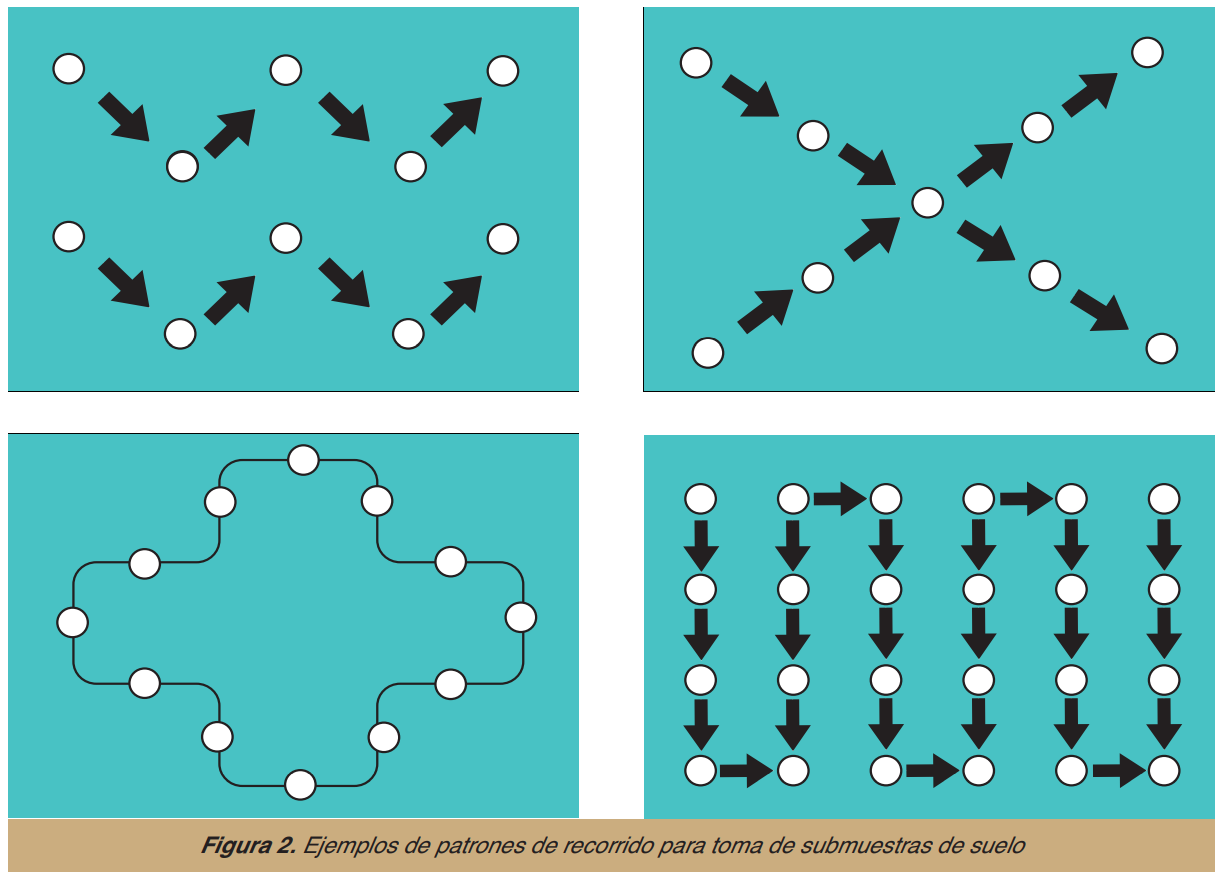
\includegraphics[width=0.3\paperwidth]{ref/sampling-patterns-srs.png}
    \caption{Patrones de muestreo para análisis de fertilidad de suelo} \footnotesize
    Fuente: Muestreo y análisis de suelos para diagnóstico de fertilidad \cite{lassaga-2011}
\end{figure}

Como se detalla más adelante, el terreno o lotes también se puede estratificar y realizar un MAS en cada estrato obtenido. El muestro sistemático por otra parte puede llegar a reducirse a un MAS o similar dado las condiciones apropiadas. Esto indica que el MAS es elemental para hacer otro tipo de diseño de muestreo.

\bigbreak

Estos son los resultados para los cálculos del MAS \cite{thompson-2012}:

\bigbreak
\textbf{Media de la población}

\bigbreak

$\overline{x}_U = \frac{1}{N}(x_1 + x_2 + ... + x_N) = \frac{1}{N} \sum \limits_{i=1}^N x_i$


\bigbreak
\textbf{Media de la muestra}

\bigbreak

$\overline{x} = \frac{1}{n}(x_1 + x_2 + ... + x_N) = \frac{1}{n} \sum \limits_{i=1}^n x_i$

\bigbreak

\textbf{Varianza de la población finita}

\bigbreak

En MAS, la varianza de la muestra $s^2$ es una estimación no-alineada de la varianza para la población finita

\bigbreak

$\sigma^2 = \frac{1}{N-1} \sum \limits_{i=1}^{N} (x_i - \overline{x}_U)^2$


\bigbreak
\textbf{Varianza de la muestra}

\bigbreak

$s^2 = \frac{1}{n-1} \sum \limits_{i=1}^n (x_i - \overline{x}_U)^2$


\bigbreak
\textbf{Total de la población}

\bigbreak

$t = \sum \limits_{i=1}^N x_i = N \overline{x}_U$


\subsection{Muestreo Sistemático}

Para realizar un muestreo sistemático se siguen los siguientes cálculos:

\bigbreak

Dado el tamaño de la población $N$ y el número de muestras $n$, hacer $k=\ceil{\frac{N}{n}}$. El valor $k$ es el período que hace que el muestreo sea sistemático. Tomar un punto aleatorio $K \in [1, k]$. Cada unidad dada por $K$, $K + k$, $K + 2k$, ... , etc., define la muestra.

\bigbreak

En ciertos casos el muestreo sistemático es el mismo MAS por lo que se pueden aplicar técnicas del MAS. Otras veces funciona como un intermediario (proxy) hacia el MAS ya que como se puede notar, si la población está dispuesta de forma aleatoria entonces lo que se tendría sería básicamente un MAS. También se debe tener en cuenta que la probabilidad de un grupo de ser escogido no es la misma como en el MAS. Otro uso que puede tener este tipo de muestreo es de hacer un trabajo similar al muestreo por clúster. De estos factores depende que la muestra sea representativa ya que si la población está ordenada de acuerdo a su índice entonces la muestra no servirá (p. ej. solo salen unidades del mismo tipo al estar ordenadas por posición, si hay hombres y mujeres solo salen hombres por ser posición par).

\bigbreak

\begin{figure}[H]
    \centering
    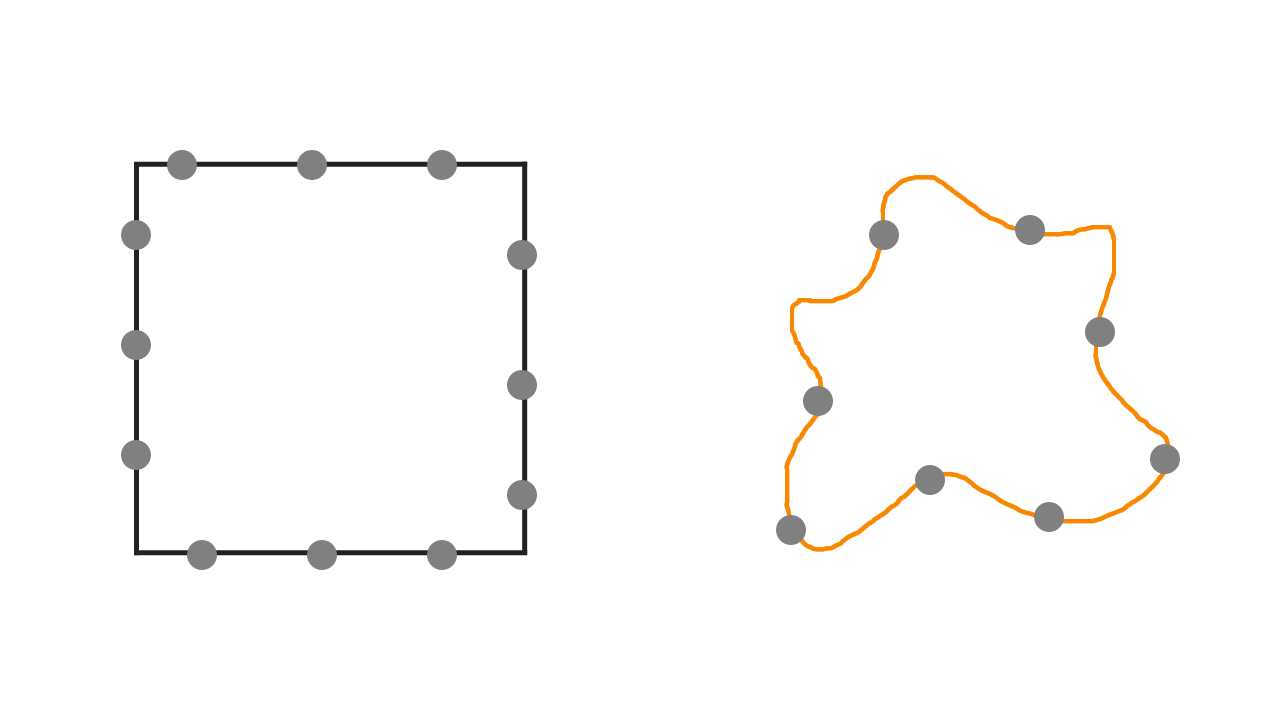
\includegraphics[width=0.3\paperwidth]{img/soil-systematic-sampling.png}
    \caption{Posible muestreo sistemático de un lote}
\end{figure}

La ilustración de arriba describe una de muchas estrategias \cite{lassaga-2011} \cite{gobpe-ministerio-del-ambiente-2014} para tomar las muestras del suelo. En este caso se toma el perímetro del suelo y sistemáticamente se toman las muestras por el perímetro, las cuales también pueden ser determinadas por otros patrones como diagonal o zigzag.

\bigbreak

Hay que tomar en cuenta que el muestreo sistemático no siempre produce una muestra representativa por lo dicho más arriba, esto es, cuando hay una distribución periódica de las unidades. Para los estudios ecológicos de suelos \cite{lohr-2009}: \say{Puede haber una topografía de crestas y surcos que daría lugar a un patrón periódico de vegetación. Si un esquema de muestreo sistemático sigue el mismo ciclo, la muestra no se comportará como una MAS}.

\subsection{Muestreo Estratificado}

Como se ha mencionado, este es uno de los temas centrales de esta investigación ya que los suelos agrícolas se pueden \textit{particionar} en lotes los cuales tienen atributos que permiten su medición y se espera poder llegar a establecerlos como homogéneos para poder elaborar el diseño del muestreo correspondiente.

\bigbreak

La población se debe de dividir (particionar) en \textbf{estratos} que sean disjuntos a dos. Esto viene de la clásica estratificación por capas. Así, para una población de tamaño $N$, se divide en $H$ estratos o capas con $N_h$ unidades en el estrato $H$. Es necesario conocer $N_1$, $N_2$, ... , $N_H$ y por tanto se tiene que $N_1 + N_2 + \cdot \cdot \cdot + N_H = N$.

\bigbreak

Para hacer un \textbf{muestreo estratificado aleatorio} como es de esperar, se toma cada estrato de $N_h$ unidades y se hacen $n_h$ mediciones aleatorias ($n_h < N_h$). Entonces el tamaño de todas las unidades de la población que se obtienen después de aplicar el muestreo se encuentra dado por $n = \sum \limits_{i=1}^H n_i$, este dato puede ser útil para dar la complejidad en espacio de la salida del muestreo virtual o de la entrada del modelo de analítica.

\bigbreak

Según la \textit{Guía de muestreo de suelo $\mid$ Gob.Pe} \cite{gobpe-ministerio-del-ambiente-2014}, el muestreo aleatorio estratificado se hace \say{cuando se dispone de información previa y el sitio presenta
características geográficas diferenciadas, es necesario estratificar o subdividir en subgrupos las
muestras que tienen homogeneidad en el terreno y en cada estrato se aplica un muestreo
aleatorio simple de manera independiente}.

\begin{figure}[H]
    \centering
    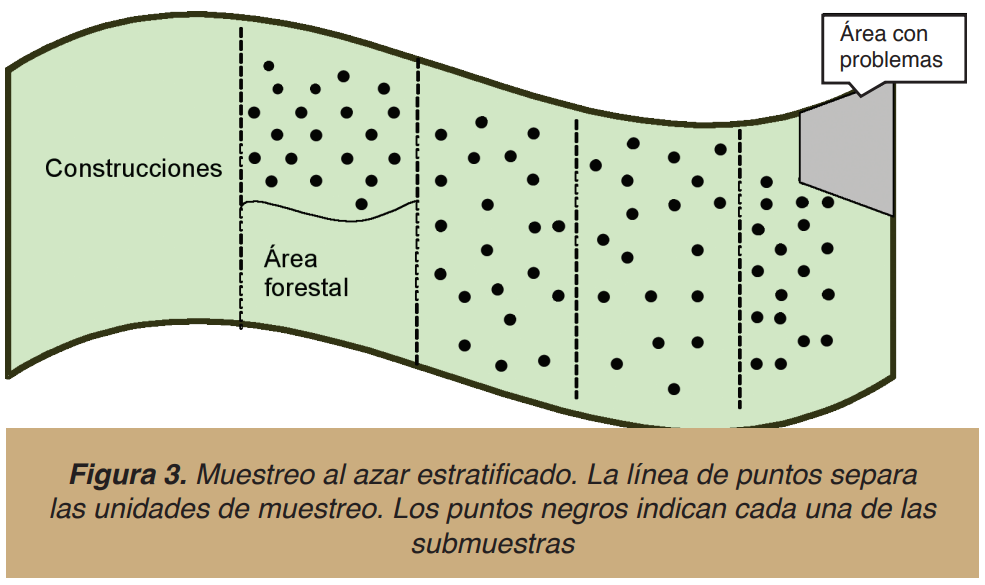
\includegraphics[width=0.3\paperwidth]{ref/stratified-sampling-examples.png}
    \caption{Ejemplo de estratos para diagnóstico de fertilidad} \footnotesize
    Fuente: Muestreo y Análisis de Suelos para Diagnóstico de Fertilidad \cite{lassaga-2011}
\end{figure}

Como resumen de los tipos de muestreos de utilidad se puede ilustrar el siguiente ejemplo:

\begin{figure}[H]
    \centering
    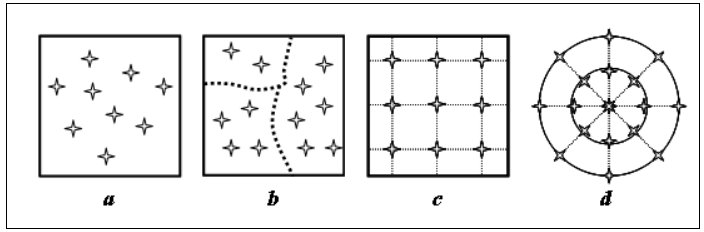
\includegraphics[width=0.3\paperwidth]{ref/kind-of-samplings-example.png}
    \caption{Ejemplo de tipos de muestreos. a) aleatorio simple, b) aleatorio estratificado, c) sistemático rejilla rectangular, d) sistemático rejilla polar} \footnotesize
    Fuente: Gobierno de México $\mid$ INNEC Instituto Nacional de Ecología y Cambio Climático \cite{innec-2007}
\end{figure}

Sea $S_h$ el conjunto de $n_h$ unidades para el estrato $H$. El valor de la unidad \textit{j}-ésima en el estrato $H$ se define como $x_{hj}$. Se siguen las siguientes valoraciones para el muestreo estratificado \cite{lohr-2009}:

\bigbreak

\textbf{Población total en el estrato H}
\bigbreak
$t_h = \sum \limits_{j=1}^{N_h} x_{hj}$


\bigbreak

\textbf{Total de la población}
\bigbreak
$t = \sum \limits_{h=1}^H t_h$


\bigbreak

\textbf{Media de la población para el estrato $H$}
\bigbreak
$\overline{x}_{hU} = \frac{\sum \limits_{j=1}^{N_h} x_{hj}}{N_h} = \frac{t_h}{N_h}$


\bigbreak

\textbf{Media de la población en general}
\bigbreak
$\overline{x}_U = \frac{\sum \limits_{h=1}^H \sum \limits_{j=1}^{N_h} x_{hj}}{N} = \frac{t}{N}$


\bigbreak

\textbf{Varianza de la población en el estrato $H$}
\bigbreak
$S_h^2 = \sum \limits_{j=1}^{N_h} \frac{(x_{hj} - \overline{x}_{hU})^2}{N_h - 1}$


\bigbreak

A partir de aquí, otros cálculos para los MAS se pueden aplicar para cada estrato. Se tiene que:

\bigbreak

$\overline{x}_h = \frac{1}{n_h} \sum \limits_{j \in S_h} x_{hj}$

\bigbreak

$s^2_h = \sum \limits_{j \in S_h} \frac{(x_{hj} - \overline{x}_h)^2}{n_h - 1}$

\bigbreak

El muestreo estratificado sin reemplazo basado en el MAS es el objetivo principal para obtener resultados bajo este marco teórico.

\subsubsection{Varianza}

Asumiendo que se tiene un muestreo estratificado donde cada estrato es relativamente homogéneo, la varianza de cada estrato es pequeña por lo que la varianza del estimado final también será pequeña, por consiguiente se sigue que \cite{gulland-1966}:

\bigbreak

Tenemos siempre que $N$ es el total de la población, $N_h$ es el $H$-ésimo estrato y $N=SN_h$. Una muestra de $n_h$ es tomada entonces del $H$-ésimo estrato, los valores que se desean estimar (longitud, peso, etc.) son dados por $x_{hj}$, $j=1,...,n_h$. De arriba, tenemos que la media estimada para el estrato $H$ es

$$
\overline{x}_h = \frac{1}{n_h} \sum \limits_{h=1}^{n_h} x_{hj}
$$

Un estimado sin sesgo de la media en toda la población es dado por esta media ponderada:

$$
\overline{x} = \frac{1}{N} \sum \limits_{h} N_h \overline{x}_h
$$

Si la varianza dentro del $H$-ésimo estrato es $S_h^2$

$$
var(\overline{x}_h) = \frac{1}{n_h} S_h^2
$$

y

$$
var(\overline{x}) = \frac{1}{N^2} \sum \frac{N_h^2}{n_h}S_h^2
$$

dado que $n_h$ sea pequeño comparado a $N_h$. Sino, las varianzas son dadas por

$$
var(\overline{x}_h) = \frac{1}{n_h}(1 - \frac{n_h}{N_h})S_h^2
$$


$$
var(\overline{x}) = \frac{1}{N^2} \sum \limits_h N_h^2 \frac{1}{n_h}(1 - \frac{n_h}{N_h})s_h^2 = \frac{1}{N^2} \sum \limits_h N_h (N_h - n_h) \frac{1}{n_h} S_h^2
$$

Esta varianza puede ser comparada con la varianza del estimado obtenido al hacer el muestreo aleatorio de la población total:

$$
var(\overline{x}') = \frac{1}{n}S^2
$$

o

$$
var(\overline{x}) = \frac{1}{n}(1 - \frac{n}{N})S^2
$$

si $n$ no es pequeño comparado con $N$ donde $S^2$ es la varianza de la población total.

\subsubsection{Ejemplo: Barco de Pesca Comercial}

En esta subsección se presenta un ejemplo con datos reales obtenido del \textit{Manual of Sampling and Statistical Methods for Fisheries Biology} \cite{gulland-1966}:

\bigbreak

La captura de un arrastrero comercial que desembarca eglefino \footnote{El eglefino es un miembro de la familia del bacalao con un sabor suave, carne firme y textura húmeda. Se usa indistintamente con el bacalao pero tiene un sabor ligeramente más dulce, lo que lo convierte en el mejor pescado blanco para ahumar. El eglefino se vende comúnmente fresco, congelado o ahumado \cite{sustainable-fishing-msc-marine-stewardship-council-2021}.} en Aberdeen \footnote{Aberdeen es una ciudad en Escocia \cite{wikipedia-aberdeen-2021}.} se clasificó en cuatro categorías de tamaño que forman los cuatro estratos. Se midieron muestras de eglefino de cada categoría y los datos resultantes se pueden resumir de la siguiente manera:

\bigbreak

% ----- TABLE

\begin{table}[H]
\centering
\begin{tabular}{|l|l|l|l|l|}
\hline
\rowcolor[HTML]{CBCEFB}
\multicolumn{1}{|c|}{\cellcolor[HTML]{CBCEFB}\textbf{Categoría}} & \multicolumn{1}{c|}{\cellcolor[HTML]{CBCEFB}\textbf{$N_h$}} & \multicolumn{1}{c|}{\cellcolor[HTML]{CBCEFB}\textbf{$n_h$}} & \multicolumn{1}{c|}{\cellcolor[HTML]{CBCEFB}\textbf{$Sx_{hj}$}} & \multicolumn{1}{c|}{\cellcolor[HTML]{CBCEFB}\textbf{$Sx_{hj}^2$}} \\ \hline
Pequeña                                                          & 2,432                                                        & 152                                                         & 5,284                                                            & 185,532                                                            \\ \hline
\rowcolor[HTML]{EFEFEF}
Pequeña-media                                                    & 1,656                                                        & 92                                                          & 3,817                                                            & 158,953                                                            \\ \hline
Media                                                            & 2,268                                                        & 63                                                          & 3,033                                                            & 146,357                                                            \\ \hline
\rowcolor[HTML]{EFEFEF}
Grande                                                           & 665                                                         & 35                                                          & 2,027                                                            & 118,169                                                            \\ \hline
\rowcolor[HTML]{FFCE93}
Total                                                            & 7,021                                                        & 342                                                         & 14,161                                                           & 609,011                                                            \\ \hline
\end{tabular}
\caption{Datos para cada estrato de la captura del barco de pesca}
\end{table}

% ----- END TABLE

donde $x$ es la longitud del pescado en $cm$.

Entonces usando como estimado de $S_h^2$ la ecuación:

$$
S_h^2 = \frac{1}{n_h - 1} \left[ \sum \limits_{h=1}^{N_h} x_{hj}^2 - \frac{1}{n_h} \left(\sum \limits_{h=1}^{N_h}x_{xj} \right)^2 \right]
$$

también tenemos que:

% ----- TABLE

\begin{table}[H]
\centering
\begin{tabular}{|l|l|l|l|l|l|}
\hline
\rowcolor[HTML]{CBCEFB}
\multicolumn{1}{|c|}{\cellcolor[HTML]{CBCEFB}\textbf{Categoría}} & \multicolumn{1}{c|}{\cellcolor[HTML]{CBCEFB}\textbf{$x_h$}} & \multicolumn{1}{c|}{\cellcolor[HTML]{CBCEFB}\textbf{$N_hx_h$}} & \multicolumn{1}{c|}{\cellcolor[HTML]{CBCEFB}\textbf{$S_{h}^2$}} & \multicolumn{1}{c|}{\cellcolor[HTML]{CBCEFB}\textbf{$\frac{S_{h}^2}{n_h}$}} & \textbf{$\frac{N_h^2S_h^2}{n_h}$} \\ \hline
Pequeña                                                          & 34.763                                                      & 84,544                                                         & 12.21                                                           & 0.0803                                                                      & 474,900                           \\ \hline
\rowcolor[HTML]{EFEFEF}
Pequeña-media                                                    & 41.489                                                      & 68,706                                                         & 6.47                                                            & 0.0703                                                                      & 192,800                           \\ \hline
Media                                                            & 48.143                                                      & 109,188                                                        & 5.48                                                            & 0.0870                                                                      & 447,500                           \\ \hline
\rowcolor[HTML]{EFEFEF}
Grande                                                           & 57.914                                                      & 38,513                                                         & 22.85                                                           & 0.6529                                                                      & 288,700                           \\ \hline
\rowcolor[HTML]{FFCE93}
Total                                                            &                                                             & 300,951                                                        &                                                                 &                                                                             & 1,403,900                         \\ \hline
\end{tabular}
\end{table}

% ----- END TABLE

Así:

\bigbreak

$\overline{x} = \frac{300,951}{7,021} = 42.9$

\bigbreak

$var(\overline{x}) = \frac{300,951}{(7,021)^2} = 0.0285$

\bigbreak

$s.d(\overline{x}) = 0.17$

\bigbreak

El $95\%$ de confianza para la longitud media real del pescado establece dicho intervalo en $42.9 \pm (2 \cdot 0.17)$ esto es, $42.6-43.2 \, cm$.

\subsection{Patrones de Muestreo}

Un patrón de muestreo se puede aplicar por ejemplo, a cada estrato de un muestreo estratificado. En el caso más trivial se puede hacer referencia a un patrón aleatorio, en otros casos se puede utilizar uno más elaborado. Esta sección recopila los patrones de muestreos de acuerdo a la \textit{Guía de muestreo de suelo $\mid$ Gob.Pe} \cite{gobpe-ministerio-del-ambiente-2014}.

\bigbreak

Los patrones de muestreo se clasifican de acuerdo a si son:  con distribución aleatoria, con distribución uniforme, con distribución heterogénea.

\subsubsection{Con Distribución Aleatoria}

Estos patrones de muestreo son utilizados en estadística.

\bigbreak

\textbf{Aleatorio:} Los puntos se escogen de forma aleatoria. Los resultados son muy irregulares.

\bigbreak

\textbf{Aleatorio sobre rejilla regular (estratificado):} El plano se divide (particiona) en zonas (estratos), se delimita una rejilla regular en todo el plano y se escoge un número igual de puntos distribuidos aleatoriamente en cada celda. Ya se ha hablado a más detalle de este patrón en secciones anteriores. La desventaja es que la forma en que están distribuidos los puntos puede ser muy dispersa, estando unos muy cerca y otros muy lejos por lo que quedan brechas de espacio vacío a menudo.

\bigbreak

\textbf{Aleatorio desalineado sobre rejilla regular:} Es una variante del patrón estratificado. En algunas celdas, la coordenada \say{x} se mueve al azar y en el resto de las celdas se mueve la coordenada \say{y}, o viceversa. La desventaja también se hereda del método estratificado.

\begin{figure}[H]
    \centering
    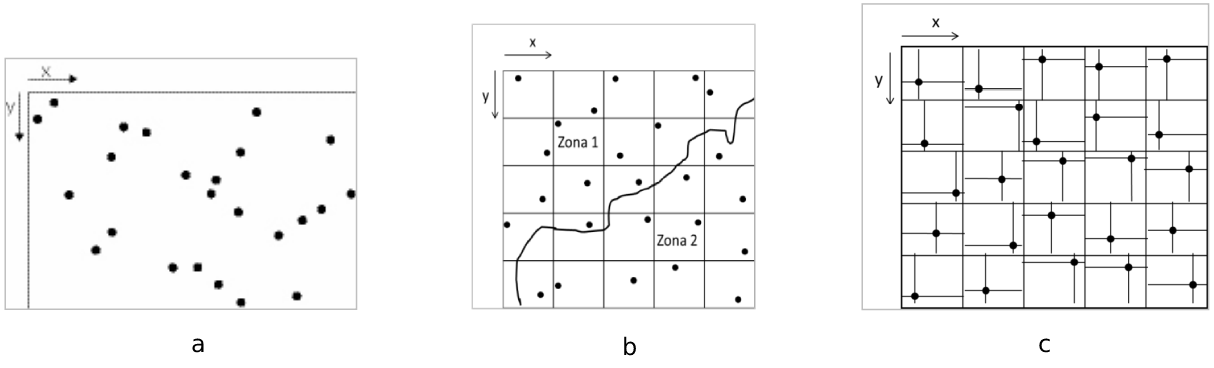
\includegraphics[width=0.3\paperwidth]{ref/random-sampling-patterns.png}
    \caption{Patrones de muestreo con distribución aleatoria} \footnotesize
    a) Aleatorio, b) Aleatorio sobre rejilla regular, c) Aleatorio desalineado sobre rejilla regular \\
    Fuente: \textit{Guía de muestreo de suelo $\mid$ Gob.Pe} \cite{gobpe-ministerio-del-ambiente-2014}
\end{figure}

\subsubsection{Con Distribución Uniforme}

\textbf{Rejillas regulares:} Se hace una rejilla de cuadrados en el plano donde cada celda es tan grande como se necesite (inversamente proporcionalmente al nivel de detalle). Por último se escoge el punto en cualquier parte de \textit{cada} celda verificando que la posición del punto sea la misma en todas las celdas.

\bigbreak

\textbf{Rejillas triangulares:} Se trazan triángulos equiláteros en el plano y se aplica el nivel de detalle establecido arriba.

\bigbreak

\textbf{Rejilla circular:} Para análisis de contaminación es de utilidad para delimitar la zona contaminada. Se trazan círculos concéntricos, separados de acuerdo al detalle requerido. Se trazan líneas rectas considerando los 8 puntos cardinales principales y se ubican los puntos de muestreo en las intersecciones. Se espera que con esta rejilla las mayores concentraciones de contaminantes se ubiquen en el centro.

\bigbreak

\textbf{Sobre una línea:} Este patrón también sirve para contaminantes cuando la contaminación siga una línea recta.

\bigbreak

\textbf{Diagonales múltiples:} Por último, con este patrón se traza una diagonal central y líneas paralelas en el plano, sobre las cuales se ubican los puntos de muestreo, manteniendo la misma distancia entre ellos.

\begin{figure}[H]
    \centering
    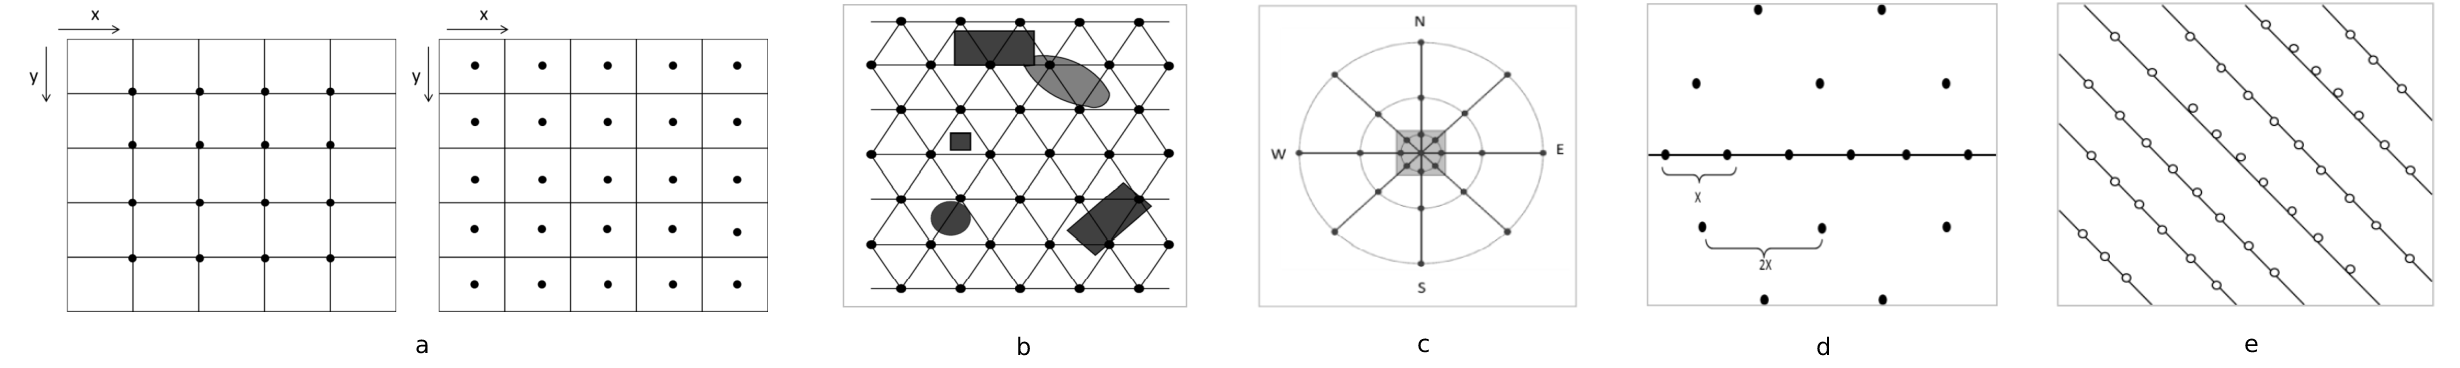
\includegraphics[width=0.4\paperwidth]{ref/uniform-sampling-patterns.png}
    \caption{Patrones de muestreo con distribución uniforme} \footnotesize
    a) Rejillas regulares, b) Rejillas triangulares, c) Rejilla circular, d) Sobre una línea, e) Diagonales múltiples \\
    Fuente: \textit{Guía de muestreo de suelo $\mid$ Gob.Pe} \cite{gobpe-ministerio-del-ambiente-2014}
\end{figure}


\subsubsection{Con Distribución Heterogénea}

Por último se enumeran este otro tipo de patrones que se pueden encontrar en un muestreo físico. Estos consisten en:

\begin{itemize}
    \item Diagonal simple
    \item Diagonales cruzadas rotantes
    \item Muestreo irregular en forma de N, S, X, o W
    \item Zig-zag
    \item Zig-zag transverso
\end{itemize}

\subsection{Muestreo Virtual}

En esta sección se documenta las diferentes salidas computacionales que son de gran importancia para trabajar con muestras de datos. Actualmente, el lenguaje de programación adoptado por la comunidad de científicos de datos y otras comunidades similares es Python debido a la estandarización que tienen sus bibliotecas de matemáticas y ciencia de datos, además de la simplicidad de su sintaxis lo cual permite la creación de prototipos y de documentos interactivos con herramientas como Jupyter Notebook \footnote{Jupyter Notebook es una aplicación web de código abierto que permite crear y compartir documentos que contienen código en tiempo real, ecuaciones, visualizaciones y texto narrativo. Los usos incluyen: limpieza y transformación de datos, simulación numérica, modelado estadístico, visualización de datos, aprendizaje automático y mucho más \cite{jupyter-2021}.}. Toda la gama de bibliotecas y herramientas para matemática y análisis de datos es dada en su mayoría bajo licencias de código abierto permisivas (comúnmente BSD-3-Clause). La ventaja de Python es que como ya se mencionó, ha sido altamente adoptado por la comunidad por su facilidad de entrada para no-programadores y también a destacar que es un lenguaje de scripting \footnote{Un lenguaje de scripting es un lenguaje de programación para un entorno de ejecución (runtime) que automatiza la ejecución de tareas que, de otro modo, serían realizadas individualmente por un operador humano \cite{wikipedia-scripting-2021B}.} por lo que su función principal es servir de interfaz (wrapper) para lenguajes de programación que suelen ser robustos, eficientes y \textit{sin abstracciones innecesarias} como C y Rust \footnote{La tendencia actual para modelos reales (no-prototipos) está empezando a emplear Rust en lugar de lenguajes similares como C y C++ y de lenguajes de entrada como Python, mostrado también por la revista Nature en \say{Why scientists are turning to Rust} \cite{nature-editorial-2020}.}.

\subsubsection{Enlaces}

Se enlistan las fuentes de los proyectos de relevancia que se necesitan para esta sección:

\begin{itemize}
    \item Python: \url{https://www.python.org}.
    \item Pandas: \url{https://pandas.pydata.org}.
    \item Matplotlib: \url{https://matplotlib.org}.
    \item GeoPandas: \url{https://geopandas.org}.
    \item NumPy: \url{https://numpy.org}.
    \item Plotly: \url{https://plotly.com}.
    \item Jupyter: \url{https://jupyter.org}.
    \item SciPy: \url{https://scipy.org}.
    \item StatsModels: \url{https://www.statsmodels.org}.
\end{itemize}

\subsubsection{Visualización de Datos}

La visualización de datos es fundamental en la ciencia de datos de forma que se puede tener mucha información de forma compacta y estudiar los resultados al mismo tiempo.

\bigbreak

Los dos usos principales de la visualización de datos son \cite{grus-2015}:

\begin{itemize}
    \item Explorar datos.
    \item Comunicar datos.
\end{itemize}

La biblioteca matplotlib es sugerida \cite{grus-2015} para la visualización de datos simples que no requieran un entorno web. Las posibilidades son: gráficos de barra simples, gráficos de líneas y gráficos de dispersión.

\bigbreak

Otras bibliotecas de interés comprenden \textbf{seaborn} derivado de matplotlib para visualizaciones más complejas y bonitas, \textbf{D3.js} para visualizaciones sostificadas e interactivas para la web, \textbf{Bokeh} para visualizaciones $3D$ en Python y \textbf{ggplot} el cual es una versión portada de la biblioteca ggplot2 del lenguaje R.

\subsubsection{Estadística}

Las bibliotecas de SciPy, pandas y StatsModels tienen una gran gama de funciones para aplicaciones de estadística. Por el resto, Python trae muchas construcciones para el manejo de funciones, vectores, operaciones y matrices aunque las matrices no son lo más fuerte de Python.

\subsubsection{GIS en la Agricultura}

Con respecto a la visualización de los datos, se tiene en consideración que el sector agrícola cuenta o debería contar con el uso de GISs. Un \textbf{GIS (Geographic Information System)} es una herramienta que crea representaciones visuales de los datos y realiza análisis espaciales a fin de tomar decisiones informadas; combina hardware, software y datos \cite{hammonds-2019}.

\bigbreak

En agricultura, un GIS puede dar información sobre el suelo, en tanto a cómo está estructurado, las propiedades y condiciones que presenta. Esto también es muy útil para visualizar un muestreo de puntos en un mapa en $2D$. Los archivos con los que se suele trabajar estos gráficos son archivos shapefile.

\bigbreak

\textbf{Shapefile:} \say{Formato de datos utilizado por la mayoría de software GIS/FMIS para almacenar datos espaciales (por ejemplo, límites de campo, ubicaciones de puntos o los polígonos que representan celdas de la cuadrícula). Un shapefile se almacena como una colección de archivos con un nombre común pero con diferentes extensiones de archivo (por ejemplo, .shp, .shx y .dbf).} Fuente: NC State Extension \cite{nc-state-extension-2021}.

\bigbreak

La biblioteca GeoPandas es una buena opción para manipular archivos shapefile y otros gráficos vectoriales.

\subsection{Encuestas Agrícolas}

A fin de obtener información precisa para poder diseñar un muestreo representativo y eficiente puede ser necesario hacer un análisis mediante encuestas y poder obtener uno de los modelos de muestreo que se conocen.

\bigbreak

Las encuestas agrícolas son muy complicadas y tienen un gran número de variables las cuales pueden comprender en tanto de \cite{organizacion-de-las-naciones-unidas-para-la-agricultura-y-la-alimentacion-1990}:

\begin{itemize}
    \item Herramientas, maquinarias, fertilizantes, plaguicidas, semillas y otros insumos.
    \item Superficie total y régimen de tenencia.
    \item Superficie bajo cultivos y producción.
    \item Verduras, frutas, nueces.
    \item Ganadería, avicultura, estabulación.

    \item Pesca, caza y explotación maderera.
    \item Regadío, pozos, avenamiento y cercado.
    \item Ingresos, comercialización, gastos, ahorros.
    \item Recuento y características de la población; mano de obra no pagada.
    \item Sanidad, educación, ocupación y estadísticas sociales de la población agrícola.
    \item Hogares y edificios agrícolas.
    \item Transporte y comunicaciones de la población agrícola.
    \item Fuentes y consumo de alimentos.
    \item Encuestas de opinión acerca de las políticas, métodos, productos, etc.
\end{itemize}

\bigbreak

Además de utilizar estas variables, se puede obtener más datos a partir de variables auxiliares. Con respecto a las fuentes de datos se puede acceder a los productores y las operaciones agrícolas, hogares agrícolas en relación con otros datos.

\bigbreak

Las encuestas agrícolas suelen ser muy variadas, cada variable que se ha enumerado tiene sus propias variaciones y propósitos múltiples. Por esto observamos que se deberá recurrir a \textbf{encuestas multitemáticas}. Además, también se necesitan aplicar métodos múltiples ya que las mediciones que se hacen requieren métodos diferentes de medición.

\subsection{Muestreo Físico}

El muestreo que se suele realizar en agricultura es probablemente para los fines de análisis de fertilidad \cite{lassaga-2011} y de contaminación \cite{gobpe-ministerio-del-ambiente-2014}. Un procedimiento estándar de acuerdo a profesionales consiste de forma básica en utilizar equipo dedicado \cite{ministry-of-agriculture-food-and-fisheries-2020} o no, dependiendo si se necesitan hacer muchos muestreos o solo es una práctica amateur. Se toman unas $6 \, pulgadas$ de tierra y se recolectan en una cubeta. Este procedimiento se ha de repetir unas $10$ a $15$ veces para que la muestra sea más uniforme a fin de obtener la muestra a partir de las múltiples submuestras mencionadas. Luego se debe de mezclar la tierra de todas las submuestras. Finalmente, se toma la cantidad de muestra especificada por el laboratorio (una bolsa) de la tierra de la cubeta ya mezclada. Se deben llenar los datos y la muestra obtenida se envía para hacer el estudio. Uno de estos datos es especificar la muestra que se manda ya que pueden haber muchas muestras que se requieren diferenciar. El procedimiento se encuentra mejor documentado en el \textit{Noble Research Institute} \cite{funderburg-2014}.

\bigbreak

Para el muestreo del diagnóstico de fertilidad se diseña una estrategia con el siguiente estilo \cite{lassaga-2011}:

\begin{itemize}
    \item Delimitar el terreno en áreas homogéneas llamadas \textbf{unidades de muestreo}. Para esto se consideran los atributos de características físicas, topográficas y similares.

    \item Contar con un plano donde se vea como se dividió el terreno y con información geográfica relevante.

    \item Otras consideraciones.
\end{itemize}

Otros registros importantes en este puto son, a saber \cite{lassaga-2011}, el \textit{rendimiento} de los cultivos por áreas homogéneas e historiales con datos anteriores.

\bigbreak

A partir de aquí, muchas estrategias de muestreo, donde ya se han mencionado algunas, se pueden aplicar para llevar a cabo este trabajo de muestreo convencional de suelo.

\subsubsection{Tipos de Errores}

Hay varios tipos de errores al tomar muestras. Adelante se muestran algunas más comunes \cite{innec-2007}. Los errores por tener un muestreo sesgado conllevan hasta pérdidas multi-billionarias \cite{gy-1998}. El siguiente caso sucedido hace ya muchas décadas es sobre una mina que fue (Pierre, 1998):

\bigbreak

\say{En un caso legal entre una mina de estaño y una fundición, se demostró que el muestreo sesgado en la fundición había infravalorado los concentrados de la mina, durante un período de varios años, en un factor de $9\%$. ¿Qué industria permitiría a sabiendas que se se va a descontar el $9\%$ del valor de sus producciones? ¿Existe alguna otra operación capaz de provocar una pérdida? ¡Nunca!}

\bigbreak

Así también hay muchos otros casos donde los errores en los muestreos han sido muy costosos. La ventaja de hoy en día es que se cuenta con mucha tecnología a diferencia de esa época.

\bigbreak

% ----- TABLE
\begin{table}[H]
\centering \tiny
\begin{tabular}{|l|l|l|}
\hline
\rowcolor[HTML]{CBCEFB}
\multicolumn{1}{|c|}{\cellcolor[HTML]{CBCEFB}\textbf{Tipo de error}}       & \multicolumn{1}{c|}{\cellcolor[HTML]{CBCEFB}\textbf{Causa}}                                                                                 & \multicolumn{1}{c|}{\cellcolor[HTML]{CBCEFB}\textbf{Forma de minimización}}                                                               \\ \hline
Fundamental                                                                & \begin{tabular}[c]{@{}l@{}}Pérdida de precisión en la muestra, \\ debido a su composición física y \\ química\end{tabular}                  & \begin{tabular}[c]{@{}l@{}}Disminución del diámetro de las partículas\\  más grandes o aumento de la masa de la\\  muestra\end{tabular}   \\ \hline
\rowcolor[HTML]{EFEFEF}
\begin{tabular}[c]{@{}l@{}}Segregación \\ y agrupación\end{tabular}        & \begin{tabular}[c]{@{}l@{}}Se debe a la distribución no al azar \\ de partículas, usualmente por efecto \\ de la gravedad\end{tabular}      & \begin{tabular}[c]{@{}l@{}}Preparación al azar de muestras compuestas\\ u homogeneización y fraccionamiento de\\  la muestra\end{tabular} \\ \hline
\begin{tabular}[c]{@{}l@{}}Heterogeneidad\\  de largo alcance\end{tabular} & Error espacial y fluctuante y no a alzar                                                                                                    & \begin{tabular}[c]{@{}l@{}}Toma de muchos incrementos para formar \\ una muestra\end{tabular}                                             \\ \hline
\rowcolor[HTML]{EFEFEF}
\begin{tabular}[c]{@{}l@{}}Heterogeneidad\\  periódica\end{tabular}        & Error de fluctuación temporal o espacial                                                                                                    & \begin{tabular}[c]{@{}l@{}}Generación correcta de muestras \\ compuestas\end{tabular}                                                     \\ \hline
\begin{tabular}[c]{@{}l@{}}Delimitación de \\ incrementos\end{tabular}     & \begin{tabular}[c]{@{}l@{}}Diseño de muestreo inapropiado y/o\\  mala selección de equipo\end{tabular}                                      & \begin{tabular}[c]{@{}l@{}}Diseño del muestreo y selección \\ apropiada de equipo\end{tabular}                                            \\ \hline
\rowcolor[HTML]{EFEFEF}
\begin{tabular}[c]{@{}l@{}}Extracción de\\  incrementos\end{tabular}       & \begin{tabular}[c]{@{}l@{}}El procedimiento de muestreo falla \\ en cuanto a la extracción precisa del\\  incremento propuesto\end{tabular} & \begin{tabular}[c]{@{}l@{}}Indispensable contar con los protocolos\\ adecuados y equipo de muestreo bien \\ diseñado\end{tabular}         \\ \hline
Preparación                                                                & \begin{tabular}[c]{@{}l@{}}Se debe a pérdidas, contaminación \\ y/o alteración de una muestra\end{tabular}                                  & \begin{tabular}[c]{@{}l@{}}Existen técnicas de campo y laboratorio\\ para evitar el problema\end{tabular}                                 \\ \hline
\end{tabular}
\caption{Tipos de errores de muestreo y técnicas para su minimización}
Fuente: Gobierno de México $\mid$ Instituto Nacional de Ecología y Cambio Climático \cite{innec-2007}
\end{table}
% ----- END TABLE

Muchas de estas soluciones para este tipo común de errores deben de ayudar a mejorar las técnicas de muestreo. Definitivamente es recomendable que el usuario que realiza la muestra física sea asesorado con estas guías las cuales se extienden mucho más allá de este estudio y son fundamentales para salvar enormes cantidades económicas y tener una ciencia de datos más correcta.


% ------------------------------ END OF  FRAMEWORK ------------------------------ %


% ------------------------------ PROPOSED PROCESS ------------------------------ %

\section{Proceso Propuesto}

Se va a enunciar a continuación un problema particular del proceso propuesto determinado por este estudio. El problema es un producto mínimo viable que funciona como artefacto de investigación. El problema consiste en una exageración donde se toma el cultivo de azúcares en Honduras (literalmente todo el territorio de Honduras) y el terreno se clasifica por departamento. Para obtener los estratos, como se ha mencionado previamente, es conveniente recurrir a las variedades por lo que será útil definir algunas variedades de azúcares. Por último se ha de elaborar el muestreo virtual y reporte de los datos obtenidos.

\bigbreak

El analista de datos deberá interpretar y generalizar este proceso en una base de caso por caso para poder aplicarlo correctamente. La etapa de analítica es muy pesada de trabajo ya que hay que abrir y definir junto con los demás interesados todo el contexto del problema. En este ejemplo se trata con cultivos de azúcar y un terreno ya predispuesto así como la selección de azúcares por variedad como estrategia de homogeneización. Todas estas condiciones van a cambiar en un caso real pero se pueden considerar abstraídas mediante estos resultados por lo que el analista de datos podrá ser capaz de generalizar.

\bigbreak

Los datos en particular se generarán de forma aleatoria al no contar con un conjunto de datos reales ya que esto estaría fuera del alcance de investigación.

\bigbreak

En los párrafos con un símbolo de implicación se dará una generalización del párrafo anterior para el analista de datos.

\subsection{Enunciado}

Asumir que en todo el territorio de Honduras se cultiva azúcar, es decir --la finca o suelo agrícola consiste en todo el territorio del país-- y se proporcionan los datos de Zafra 2021. Mediante un SIG se ha obtenido un mapa del área clasificada por departamento, en total, 18 departamentos.

\bigbreak

$\implies$ El analista de datos en esta etapa deberá contar con la muestra física y el modelo del suelo agrícola probablemente en formato shapefile (shp). Por tanto, el conjunto de datos puede comprender a cualquier tipo de  cultivo además de azúcar y cualquier zona geográfica que deberá tener
cierta delimitación geográfica.

\bigbreak

A fin de obtener los estratos se ha establecido usar la variedad --variable que define propiedades biológicas de los cultivos-- para clasificar el suelo. Al ser cosecha de azúcar, se asume que se cultivan las variedades:

\begin{itemize}
    \item Ninguna
    \item CP 72-2086
    \item Mex 69-290
    \item Mex 79-431
    \item ITV 92-1424
\end{itemize}

Las cuales son variedades muy conocidas.

\bigbreak

$\implies$ El analista obtendrá una lista mucho más grande de variedades disponibles en el suelo.

\bigbreak

Se debe de obtener un muestreo físico con la siguiente estructura mínima:

\begin{itemize}
    \item Estrato
    \item Área Cosechada (HA)
    \item TA/HA Real
\end{itemize}

Donde el conjunto de datos representa los registros tomados por el usuario en ese año de zafra.

\subsection{Análisis Geográfico}

Este proceso consiste en un análisis del SIG estándar. Se definen las constantes, se carga el archivo shapefile y se le da formato correspondiente agregando demás columnas. Se identifica como variable independiente a la columna departamento.

\bigbreak

El análisis del SIG da un reporte de alto nivel sobre el muestreo físico. Luego se carga el \textit{DataFrame} del muestreo físico para zafra año 2021 en este caso, entonces se desarrolla el MAS Estratificado y se establece el reporte del muestreo obtenido. Con esto, se puede hacer finalmente un análisis de fertilidad consistente y más eficiente. Por tanto, el análisis geográfico es la de las tres etapas mencionadas.

\subsubsection{Recopilación de Datos}

Este problema es una exageración que permite de momento llevar a cabo el proceso propuesto de muestreo virtual. La mayor parte de datos creados en este problema no tienen relación con la realidad pero si sirven como modelo para ser aplicado a un caso con datos reales.

\bigbreak

Los datos del muestreo físico son recolectados mediante la desnormalización de la base de datos del usuario. Esto implica que en análisis de datos se ven muchos fenómenos como redundancia, etc. El cultivo de azúcares se da por zafra, en este caso, se asume una zafra 2021 la cual da todos los registros de ese año.

\bigbreak

Las 4 \href{https://www.gob.mx/conadesuca/es/articulos/variedades-de-cana-de-azucar?idiom=es}{variedades} tomadas son una referencia importante que se encontrará de forma mucho más diversa en una base de datos real. Estas son variedades significativas, en un caso real se tiene una gran cantidad de variedades de azúcares por lo que el analista deberá tomar solo aquellas significativas para reducir la carga de la muestra. Otras variedades de azúcares significativas incluye, a saber, \textit{CP 73-1547}, \textit{RB 86-7515}, etc. Las encuestas pueden ser herramientas adecuadas para la obtención de esta información por parte de los interesados.

\bigbreak

Por tanto, se debe de tomar una variable adecuada física o biológica como la variedad del cultivo para crear cada estrato con unidades de muestreo homogéneas. Al definir inicialmente los estratos, se tendrá una lista muy grande de opciones por lo que será necesario tomar un subconjunto significativo de estos estratos filtrando aquellos que no son significativos de acuerdo al criterio establecido por el analista. Después de este filtrado, se obtienen los estratos definitivos y el mapa original queda con áreas no representativas por lo que se define el estrato vacio \textit{Ninguno}. Originalmente puede que ya existan áreas no representativas como zonas de construcción, contaminadas, etc.

\subsubsection{Filtrado}

El filtrado inicial se ha definido como sigue:

\begin{itemize}
    \item Remover estratos vacíos.
    \item Remover estratos con variedades insignificantes.
\end{itemize}

Para determinar las variedades insignificantes se establece una cota mínima (umbral) de área cosechada por variedad, estos datos vienen del muestreo físico. Por tanto, la condición para determinar si una variedad es significante es si pertenece a las cuatro variedades definidas arriba o si el área cosechada para esa variedad supera un umbral determinado. En este problema solo se filtrará tomando las cuatro variedades comúnes.

\subsection{Muestreo Físico}

Este \textit{DataFrame} contiene los supuestos datos de zafra $2021$ en el suelo agrícola. Es decir, todos los registros de variedades tomados en ese año. Además, en un conjunto de datos original existen muchas otras variables que pueden ser usadas para otros cálculos. Este \textit{DataFrame} solo contiene el filtrado con las columnas correspondientes para el análisis de rendimiento.

\subsection{Resumen de Muestro}

En las siguientes dos tablas se listan los datos del SIG y del muestreo físico filtrado para análisis de rendimiento correspondientemente.

\subsubsection{Modelo de Muestreo}

\textbf{Muestro Físico}

\bigbreak

El tamaño de la población $N = 5,000$ unidades de muestreo.

\bigbreak

Unidad de área: Hectárea.

\bigbreak

\textbf{Muestreo Virtual}

\bigbreak

\textbf{Estratos}

\bigbreak

Se han definido cuatro estratos significativos correspondientes a variedades de azúcares y uno vacío. Por tanto, $H = \{ Ninguno, H_1, ... , H_4 \}$.

\bigbreak

Tamaño de muestreo por estrato $(H_n) = t_h * factor$ donde \textit{factor} en $[0,1]$ representa el porcentaje de unidades aleatorias a tomar en cada estrato $H$ respecto a $t_h$.

\bigbreak

Con respecto al conjuntos de datos geográficos originalmente cargado, este simplemente cuenta con una (generosa) columna \textit{geography} la cual contiene la información vectorial del mapa del suelo agrícola. También fue útil la columna \textit{DEPARTMENT\_COL} conteniendo la partición hecha por el usuario. En este caso, los estratos son por variedad significante por lo que el problema debe ser tal que los subconjuntos de la partición del mapa (\say{departamentos}) contienen únicamente una variedad. Esto se detalla más en la sección de visualización abajo. A partir de estos criterios, el analista deberá poder obtener la información geográfica útil del usuario.

\subsection{Visualización de Muestro}

En los siguientes bloques se visualizan los datos obtenidos arriba.

\bigbreak

Por ejemplo, en los \say{departamentos} en azul (Cortés, Atlántida, Yoro,Ocotepeque, Lempira y El Paraíso) se cultiva variedad \textit{CP 72-2086}. Así, esos $6$ \say{departamentos} forman un estrato.

\subsection{Modelo}

El resultado del muestreo virtual se desarrolla en esta sección.

\bigbreak

Se importa el módulo de muestreo que contiene la implementación del modelo de muestreo virtual y el módulo que contiene el caso de prueba para resolución:

\bigbreak

\begin{lstlisting}[language=Python, caption=Importar dependencias]
import sampling
from test import main
\end{lstlisting}

\bigbreak

Se crea una instancia del problema conteniendo la información geográfica y muestreo físico generado con datos aleatorios. Recordar que cada vez al correr el programa se genera un problema con nuevos datos y que los datos generados aleatoriamente no producen resultados comparables a la realidad pero el proceso es totalmente válido para cualquier caso de uso tanto de prueba como real.

\bigbreak

\begin{lstlisting}[language=Python, caption=Importar dependencias]
main = main.Main.new_instance('./test')
sampling = sampling.Sampling.from_main(main)
\end{lstlisting}

\bigbreak

Imprimiendo el muestreo físico se obtuvo el conjunto de datos siguiente:

\begin{table}[H]
    \centering
    \begin{tabular}{|l|l|l|l|}
    \hline
    \rowcolor[HTML]{CBCEFB}
    \textbf{} & \textbf{Estrato} & \textbf{Área Cosechada (HA)} & \textbf{TA/HA Real} \\ \hline
    0         & CP 72-2086       & 1730.4                       & 8.6                 \\ \hline
    \rowcolor[HTML]{EFEFEF}
    1         & ITV 92-1424      & 325.6                        & 1.2                 \\ \hline
    2         & Ninguno          & 2414.6                       & 9.8                 \\ \hline
    \rowcolor[HTML]{EFEFEF}
    3         & CP 72-2086       & 3867.4                       & 9.9                 \\ \hline
    4         & Mex 69-290       & 1683.8                       & 4.2                 \\ \hline
    \end{tabular}
    \caption{Primeros datos del muestreo físico generado}
\end{table}

Donde como se estableció en el planteamiento del problema, este \textit{DataFrame} contiene $5,000$ registros.

\bigbreak

En el siguiente bloque es donde se debe configurar el modelo para que realice el muestreo:

\bigbreak

\begin{lstlisting}[language=Python, caption=Configurar el muestreo virtual]
# Configurar muestreo
sampling.stratum_sampling_size(400)

# Configurar filtr de estratos
stratum_filter = sampling.stratum_filter()
stratum_filter.area_threshold(2_480_000)

# Correr modelo de muestreo virtual
result = sampling.run()
sampled_df = result.sampling()

result.show_sampling()
result.show_stratum_filter()
\end{lstlisting}

\bigbreak

Para futuras versiones se tendrá en cuenta que se debería poder pasar el vector que define el tamaño de la muestra para cada estrato en lugar de pasar un único tamaño de la muestra para todos los estratos. Esto es, $n_h < N_h$ debería ser seleccionado para cada estrato. El resultado del muestreo da:

\begin{table}[H]
    \centering
    \begin{tabular}{|l|l|l|l|}
    \hline
    \rowcolor[HTML]{CBCEFB}
    \textbf{} & \textbf{Estrato}                                          & \textbf{Área Cosechada (HA)} & \textbf{TA/HA Real} \\ \hline
    0         & \cellcolor[HTML]{FFFFFF}{\color[HTML]{171717} CP 72-2086} & 4773.5                       & 1.4                 \\ \hline
    \rowcolor[HTML]{EFEFEF}
    1         & {\color[HTML]{171717} CP 72-2086}                         & 2341.9                       & 5.6                 \\ \hline
    2         & \cellcolor[HTML]{FFFFFF}{\color[HTML]{171717} CP 72-2086} & 148.7                        & 6.9                 \\ \hline
    \rowcolor[HTML]{EFEFEF}
    3         & {\color[HTML]{171717} CP 72-2086}                         & 1794.2                       & 0.6                 \\ \hline
    4         & \cellcolor[HTML]{FFFFFF}{\color[HTML]{171717} CP 72-2086} & 2061.7                       & 3.3                 \\ \hline
    ...       & ...                                                       & ...                          & ...                 \\ \hline
    795       & \cellcolor[HTML]{FFFFFF}{\color[HTML]{171717} Mex 79-431} & 899.8                        & 0.9                 \\ \hline
    \rowcolor[HTML]{EFEFEF}
    796       & {\color[HTML]{171717} Mex 79-431}                         & 4232.5                       & 8.9                 \\ \hline
    797       & \cellcolor[HTML]{FFFFFF}{\color[HTML]{171717} Mex 79-431} & 827.2                        & 7.5                 \\ \hline
    \rowcolor[HTML]{EFEFEF}
    798       & {\color[HTML]{171717} Mex 79-431}                         & 2025.5                       & 6.6                 \\ \hline
    799       & \cellcolor[HTML]{FFFFFF}{\color[HTML]{171717} Mex 79-431} & 4332.8                       & 4.6                 \\ \hline
    \end{tabular}
    \caption{Resultado del muestreo virtual}
\end{table}

El cual contiene $800$ registros que se comprobará que son representativos. Esto comparado a los $5,000$ registros originales. Notar que los datos se han agrupado por variedad en el resultado.

\bigbreak

Además de esto, el modelo también produce un reporte para ver el filtrado inicial que se hizo para filtrar todos aquellos estratos insignificantes. De acuerdo al valor de umbral asignado al algoritmo se obtuvieron que solo esos dos estratos son significantes:

\begin{figure}[H]
    \centering
    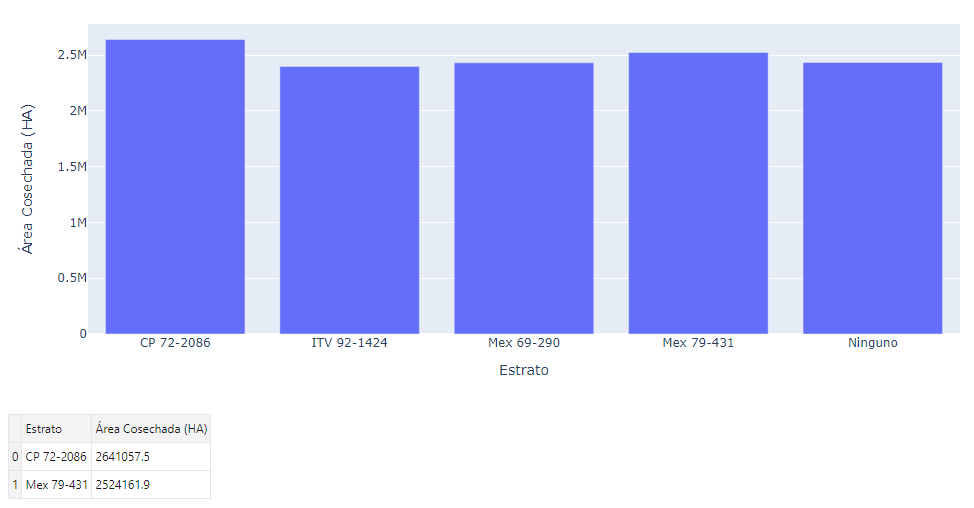
\includegraphics[width=0.3\paperwidth]{img/process-stratum-filter-report.png}
    \caption{Resultado del filtro de estratos}
\end{figure}

Por lo que las variedades (\textit{ITV 92-1424
}, $2.39938M$), (\textit{Mex 69-290}, $2.431765M$) y (\textit{Ninguno}, $2.435103M$) quedan fuera definitivamente del conjunto de datos al ser insignificantes por tener un valor de área cosechada menor al umbral establecido. Aquí también se considerará para el modelo filtrar siempre el estrato \textit{Ninguno} pero de momento, aún se toma en cuenta. En un caso real, habrán muchos más estratos y se verá que muchos son claramente insignificantes.

\bigbreak

Al tener los resultados, el analista debe poder verificar la efectividad del modelo. Esto se demuestra a continuación. Se utilizó el análisis de rendimiento como aplicación del muestro virtual.

\bigbreak

\begin{lstlisting}[language=Python, caption=Análisis de rendimiento]
# Rendimiento
def get_yield(df):
    grouped = df.groupby(hn.STRATUM_COL)
    abs_yield = grouped[hn.HardSampling.YIELD_COL].sum().reset_index()
    abs_areas = grouped[hn.HardSampling.HARVESTED_AREA_COL].sum().reset_index()
    yield_result = abs_yield.merge(abs_areas)
    yield_result["Rendimiento"] = abs_yield[hn.HardSampling.YIELD_COL] / abs_areas[hn.HardSampling.HARVESTED_AREA_COL]
    return yield_result
\end{lstlisting}

\bigbreak

Notar que se suman los valores de rendimiento y de área cosechada agrupado como estratos lo que da valores absolutos y luego se toma un valor ponderado como el rendimiento de cada variedad.

\bigbreak

Por último, se mide el error relativo al computar el rendimiento del conjunto de datos originales contra el conjunto de datos del muestro virtual:

\bigbreak

\begin{lstlisting}[language=Python, caption=Comprobación de la eficiencia del muestro virtual obtenido]
sampled_yield = get_yield(sampled_df)
real_yield = get_yield(hard_sampling)

sampled_yield['Rendimiento real'] = real_yield['Rendimiento']
sampled_yield['Error relativo (%)'] = (abs(sampled_yield['Rendimiento'] - real_yield['Rendimiento']) / real_yield['Rendimiento']) * 100
\end{lstlisting}

\bigbreak


\begin{table}[H]
    \tiny
    \centering
    \begin{tabular}{|l|l|l|l|l|l|l|}
    \hline
    \rowcolor[HTML]{CBCEFB}
      & Estrato    & \begin{tabular}[c]{@{}l@{}}TA/HA \\ Real\end{tabular} & \begin{tabular}[c]{@{}l@{}}Área Cosechada\\  (HA)\end{tabular} & Rendimiento & \begin{tabular}[c]{@{}l@{}}Rendimiento \\ Real\end{tabular} & \begin{tabular}[c]{@{}l@{}}Error \\ Relativo (\%)\end{tabular} \\ \hline
    0 & CP 72-2086 & 1947.6                                                & 960109.2                                                       & 0.0020285   & 0.0020283                                                   & 0.0086127                                                      \\ \hline
    \rowcolor[HTML]{EFEFEF}
    1 & Mex 79-431 & 1914.0                                                & 979276.8                                                       & 0.0019545   & 0.0020501                                                   & 4.6667605                                                      \\ \hline
    \end{tabular}
    \caption{Comparación de muestreo físico contra muestreo virtual}
\end{table}

Si el tamaño de muestra por estrato se baja a un valor demasiado pequeño el error relativo se vuelve muy grande en magnitudes de $20-150\%$ por lo cual esta es una forma de comprobar la configuración correcta del muestreo virtual.

\bigbreak

Con esta configuración el analista podrá desplegar a producción datos históricos correctamente muestreados incrementado significativamente el tiempo de ejecución de los modelos de ciencia de datos que toman como alimento estos datos históricos y que probablemente se actualizan a menudo y corren periódicamente en la nube la cual además puede tener limitaciones de recursos.

\section{Conclusiones}

Se desarrolló un modelo de muestro virtual para suelo agrícola que consiste en una herramienta mínima viable como artefacto de investigación. El modelo implementó una API que es de utilidad para el analista de datos y puede ser configurada y extendida en funcionalidad.

\bigbreak

Se desarrolló un marco teórico para entender mejor ambas partes interesadas, a saber, la empresa de analítica y agrícola con cierto enfoque en Honduras. Esto sirve al analista a poder configurar el modelo de muestreo y obtener información clave sobre como definir los estratos y la obtención del SIG del suelo apropiada para la visualización del muestreo. Se ha tomado en cuenta el uso de encuestas como herramienta de análisis de sistemas para lograr este objetivo.

\bigbreak

Finalmente, se demostró el funcionamiento y eficiencia del prototipo con datos irreales y sin mucho sentido debido a las complicaciones para obtener un conjunto de datos real de acceso libre. Esto indica que el analista puede generalizar el proceso de muestreo en una base de caso por caso y que al aplicar la herramienta de muestreo será de utilidad para un caso de uso real.

\subsection{Recomendaciones}

Una vez aplicados los conocimientos y resultados de la tesis se recomienda:

\begin{itemize}
    \item Proyecto en \href{https://github.com/tobiasbriones/cp-unah-mm700-agricultural-soil-sampling-for-data-analysis}{GitHub}.

    \item Dar uso a la POO para crear APIs que sean útiles y reutilizables.

    \item Extender el modelo con cálculos estadísticos para reportar y automatizar la selección de valores (e.g. $h_n$).

    \item Crear más documentación de alto nivel para entender el proceso de muestreo al trabajar en equipo y crear aplicaciones.
\end{itemize}

\section{Reconocimientos}

Se agradece al equipo de \textit{PL Intelligent Solutions Co} por las visiones dadas sobre el contexto e importancia del problema de investigación en el país.


% ------------------------------ END OF PROPOSED PROCESS ------------------------------ %


\section{Anexos}

Se ha tomado nota en pequeña parte sobre la elaboración y estructura de \textit{Manual de Elaboración y Presentación de Tesis} \cite{universidad-san-carlos-2016}, \textit{Metodología de la investigación} \cite{collado-2014}, \textit{Introducción a la metodología de la investigación científica} \cite{cabezas-2018} para la propuesta inicial de investigación.

\subsection{Glosario}

\begin{itemize}
    \item \textbf{Analítica:} Proceso de detectar, interpretar y comunicar patrones significativos en los datos, así como usar herramientas para que toda la organización pueda realizar cualquier pregunta sobre cualquier información en todos los entornos y dispositivos posibles \cite{oracle-2021}.

    \item \textbf{Rendimiento:} Razón con unidad dimensional [MASA][PRODUCTO]/[ÁREA] útil para medir el beneficio producido en una zafra (p. ej. 1TA/HA 1 tonelada de azucar por hectárea).

    \item \textbf{Zafra:} Cosecha de la caña dulce (p. ej. zafra 2020-2021).
\end{itemize}

\subsubsection{Términos de Dominio Específico}

\begin{itemize}
    \item \textbf{Usuario:} Empresa agrícola en Honduras.

    \item \textbf{Usuario interno:} Empleado de la empresa agrícola.

    \item \textbf{Muestreo físico:} Muestra original que el usuario tomó en su suelo agrícola.

    \item \textbf{Muestreo virtual:} Resultado o salida del modelo que se ha de desarrollar en este estudio el cual tiene como entrada el muestreo físico.

    \item \textbf{Curar:} Transformar los datos originales mediante filtros de forma que se eliminen los todos aquellos datos innecesarios o corruptos para el análisis subyacente.
\end{itemize}


\subsection{Introducción}

\begin{lstlisting}[language=Python, caption=Introducción al enunciados del problema]
from main import plot
from test import hn_example as hn

# ----------

hn_gis = hn.Gis()

hn_gis.parent_dir = './test'

# ----------

# SIG

hn_gdf = hn_gis.load()
hn_df = hn_gis.df()

hn_df

# ----------

# Muestreo fisico (generado aleatoriamente)

hard_sampling = hn.HardSampling.generate()

hard_sampling

# ----------

# SIG

plot(hn_gdf, 'Mapa de Suelo Agricola por Lotes', size=20)

# Mapa de Suelo Agricola por Estratos
hn_gdf.plot(figsize=(20, 20), column=hn.STRATUM_COL, legend=True)

# ----------

from test import main
import sampling

main = main.Main.new_instance('./test')
sampling = sampling.Sampling.from_main(main)
sim = sampling.new_sampling_simulator()

sampling.stratum_sampling_size(300)

sim.simulate(hn.Stratum.CP_72_2086)
\end{lstlisting}

\begin{figure}[H]
    \centering
    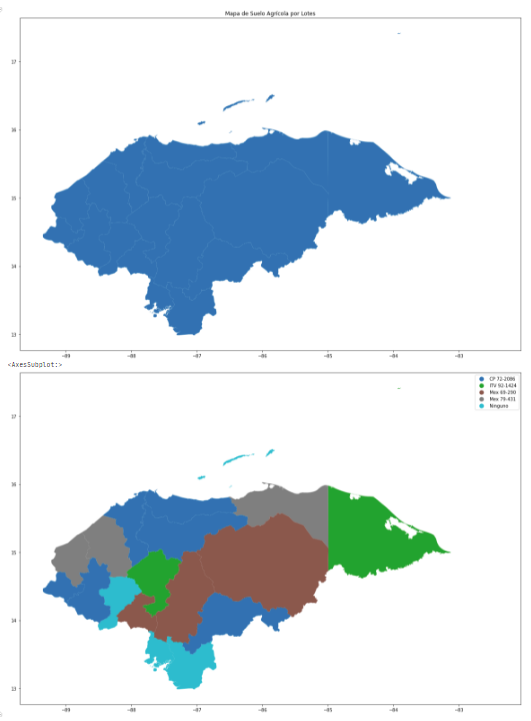
\includegraphics[width=0.3\paperwidth]{ref/intro-fig-1.png}
    \caption{Mapa del suelo agrícola}
    Fuente: Derivado de GADM data (version 3.6) \cite{gadm-2021}
\end{figure}

\begin{figure}[H]
    \centering
    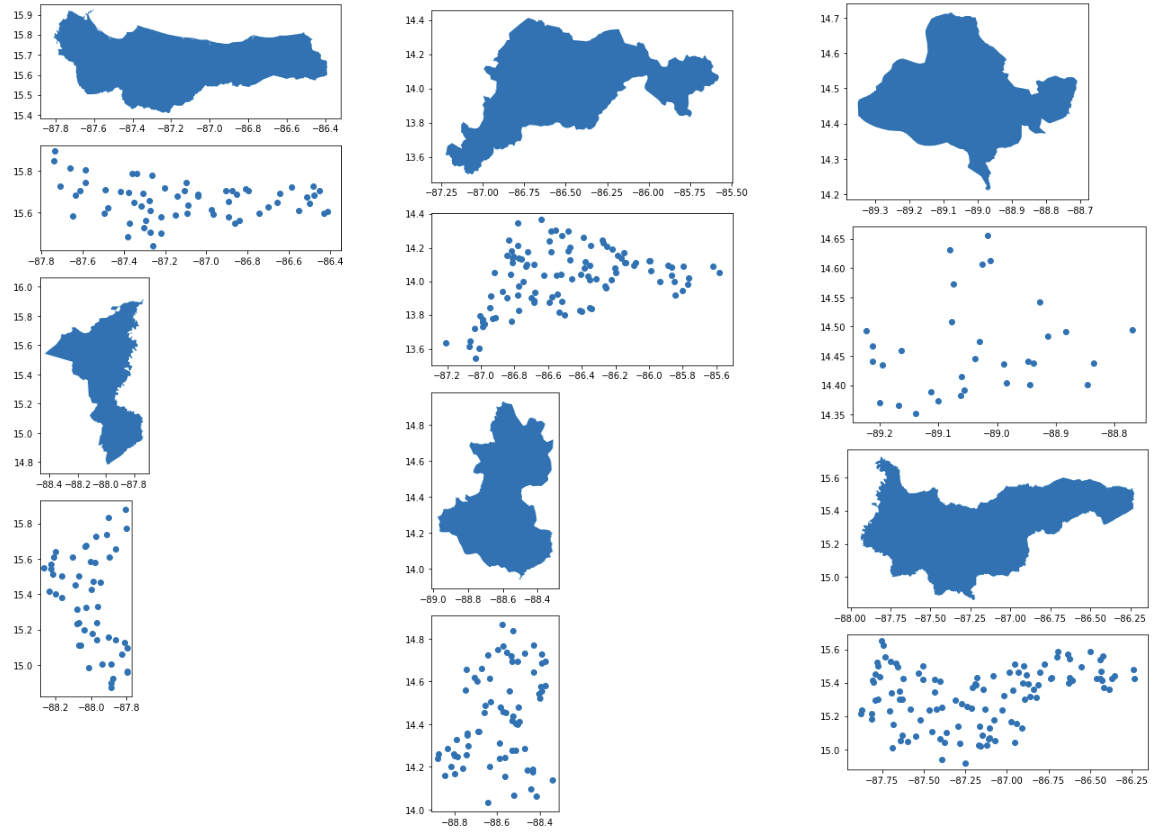
\includegraphics[width=0.3\paperwidth]{ref/intro-fig-2.png}
    \caption{Simulación de muestreo virtual para el estrato $CP \,\, 72-2086$}
    Fuente: Derivado de GADM data (version 3.6) \cite{gadm-2021}
\end{figure}

\subsection{Código fuente}

Se recomienda obtener una copia del código fuente desde el proyecto en GitHub dado en las recomendaciones. Sin embargo, se adjunta una copia ligera sin documentación a continuación.


\bigbreak

\begin{lstlisting}[language=Python, caption=test/main.py]
from . import hn_example as hn

DEF_STRATUM_COL = 'Estrato'

class Main:
    @staticmethod
    def new_instance(parent_dir='.'):
        gis = hn.Gis(parent_dir)
        df = hn.HardSampling.generate()

        gis.load()
        return Main(gis, df)

    def __init__(self, gis, df):
        self.__gis = gis  # Immutable
        self.__df = df  # Immutable

    def gis(self):
        return self.__gis

    def gdf(self):
        return self.__gis.gdf()

    def df(self):
        return self.__df

    def cols(self):
        return cols()

    def filter(self):
        valid_stratum = self.__df[DEF_STRATUM_COL] != hn.Stratum.NONE
        self.__df = self.__df[valid_stratum].reset_index(drop=True)


class ColumnConfig:
    def __init__(
        self,
        stratum='stratum',
        harvested_area='harvested_area',
        gis_area='area',
        gis_subset='subset'
    ):
        self.stratum = stratum
        self.harvested_area = harvested_area
        self.gis_area = gis_area
        self.gis_subset = gis_subset


def cols():
    return ColumnConfig(
        stratum=hn.STRATUM_COL,
        harvested_area=hn.HardSampling.HARVESTED_AREA_COL,
        gis_area=hn.Gis.AREA_COL,
        gis_subset=hn.Gis.DEPARTMENT_COL
    )
\end{lstlisting}




\bigbreak





\begin{lstlisting}[language=Python, caption=test/hn\_example.py]
import random
import functools
import numpy as np
import pandas as pd
import geopandas as gpd
from strenum import StrEnum

STRATUM_COL = 'Estrato'

class Stratum(StrEnum):
    NONE = 'Ninguno'
    CP_72_2086 = 'CP 72-2086'
    MEX_69_290 = 'Mex 69-290'
    MEX_79_431 = 'Mex 79-431'
    ITV_92_1424 = 'ITV 92-1424'


class Gis:
    FILE_NAME = '/data/gis/gadm36_HND_1.shp'
    DEPARTMENT_COL = 'NAME_1'
    AREA_COL = 'Area Departamento (HA)'

    def __init__(self, parent_dir='.'):
        self.parent_dir = parent_dir
        self.__gdf = gpd.GeoDataFrame()

    def df(self):
        data = self.__gdf.drop(columns='geometry')
        return pd.DataFrame(data)

    def gdf(self):
        return self.__gdf

    def load(self):
        df = Gis.get_df()
        gdf_data = gpd.read_file(self.parent_dir + Gis.FILE_NAME)
        self.__gdf = gpd.GeoDataFrame(df, geometry=gdf_data.geometry)
        return self.__gdf

    @staticmethod
    def get_df():
        departments = [
            'Atlantida',
            'Choluteca',
            'Colon',
            'Comayagua',
            'Copan',
            'Cortes',
            'El Paraiso',
            'Francisco Morazan',
            'Gracias a Dios',
            'Intibuca',
            'Islas de la Bahia',
            'La Paz',
            'Lempira',
            'Ocotepeque',
            'Olancho',
            'Santa Barbara',
            'Valle',
            'Yoro'
        ]

        strata = [
            Stratum.CP_72_2086,
            Stratum.NONE,
            Stratum.MEX_79_431,
            Stratum.ITV_92_1424,
            Stratum.MEX_79_431,
            Stratum.CP_72_2086,
            Stratum.CP_72_2086,
            Stratum.MEX_69_290,
            Stratum.ITV_92_1424,
            Stratum.NONE,
            Stratum.NONE,
            Stratum.MEX_69_290,
            Stratum.CP_72_2086,
            Stratum.CP_72_2086,
            Stratum.MEX_69_290,
            Stratum.MEX_79_431,
            Stratum.NONE,
            Stratum.CP_72_2086
        ]

        areas_km2 = [
            4227,
            4397,
            8875,
            5120,
            3239,
            3911,
            7383,
            8619,
            15876,
            3126,
            229,
            2534,
            4285,
            1636,
            24038,
            5013,
            1618,
            7787
        ]

        areas_ha = list(map(lambda a: a * 100, areas_km2))

        return pd.DataFrame({
            Gis.DEPARTMENT_COL: departments,
            STRATUM_COL: strata,
            Gis.AREA_COL: areas_ha
        })


class HardSampling:
    YIELD_COL = 'TA/HA Real'
    HARVESTED_AREA_COL = 'Area Cosechada (HA)'
    POPULATION_SIZE = 100_000

    @staticmethod
    def generate():
        variety_data = pd.DataFrame(
            random.choices(
                list(Stratum),
                k=HardSampling.POPULATION_SIZE
            ),
            columns=[STRATUM_COL]
        )
        area_data = pd.DataFrame(
            np.random.randint(
                0.1,
                50_000,
                (HardSampling.POPULATION_SIZE, 1)
            ) / 10,
            columns=[HardSampling.HARVESTED_AREA_COL]
        )
        yield_data = pd.DataFrame(
            np.random.randint(0, 100, (HardSampling.POPULATION_SIZE, 1)) / 10,
            columns=[HardSampling.YIELD_COL]
        )
        data = [variety_data, area_data, yield_data]
        return functools.reduce(
            lambda left, right: pd.merge(
                left,
                right,
                left_index=True,
                right_index=True
            ),
            data
        )
\end{lstlisting}





\bigbreak




\begin{lstlisting}[language=Python, caption=sampling.py]
import random
import numpy as np
import pandas as pd
import geopandas as gpd
import plotly.express as px
from IPython.core.display import display

DEF_STRATUM_SAMPLING_SIZE = 1_000

class Sampling:
    @staticmethod
    def from_main(main):
        return Sampling(main.gis(), main.df(), main.cols())

    def __init__(self, gis, df, cols):
        self.__gis = gis  # Immutable
        self.__df = df  # Immutable
        self.__cols = cols  # Immutable
        self.__n = DEF_STRATUM_SAMPLING_SIZE
        self.__stratum_filter = StratumFilter(df, cols)

    def stratum_sampling_size(self, value):
        self.__n = value

    def stratum_filter(self):
        return self.__stratum_filter

    def run(self):
        sampling = pd.DataFrame(self.__df, copy=True)

        sampling = self.__stratum_filter.filter_df(sampling)
        sampling = self.__stratified_random_sampling(sampling)
        sampling = sampling.reset_index(drop=True)
        return Result(
            sampling,
            self.__stratum_filter
        )

    def new_sampling_simulator(self):
        return SamplingSimulator(self.__n, self.__cols, self.__gis)

    def __stratified_random_sampling(self, df):
        grouped = df.groupby(self.__cols.stratum)
        sampled_strata = []

        for name, group in grouped:
            stratum_df = group.reset_index(drop=True)
            sample = self.__random_sampling(stratum_df)
            sampled_strata.append(sample)
        return pd.concat(sampled_strata)

    def __random_sampling(self, stratum_df):
        h_n = stratum_df[stratum_df.columns[0]].count()
        units = random.sample(range(0, h_n - 1), self.__n)
        return stratum_df.filter(items=units, axis=0)


class Result:
    def __init__(
        self,
        sampling,
        stratum_filter
    ):
        self.__sampling = sampling
        self.__stratum_filter = stratum_filter

    def sampling(self):
        return self.__sampling

    def show_sampling(self):
        display(self.__sampling)

    def show_stratum_filter(self):
        self.__stratum_filter.plot_stratum_areas()
        display(self.__stratum_filter.result())


class StratumFilter:
    def __init__(self, df, cols):
        self.__df = df
        self.__cols = cols
        self.__area_threshold = 0
        self.__result = pd.DataFrame()

    def area_threshold(self, value):
        self.__area_threshold = value

    def result(self):
        return self.__result

    def filter_df(self, df):
        self.filter()
        strata = self.to_list()
        significant_stratum = df[self.__cols.stratum].isin(strata)
        return df[significant_stratum]

    def filter(self):
        areas = self.stratum_areas()
        curated = areas[
            areas[self.__cols.harvested_area] > self.__area_threshold
            ]
        self.__result = curated.reset_index(drop=True)
        return self.__result

    def to_list(self):
        return list(self.__result[self.__cols.stratum])

    def plot_stratum_areas(self):
        fig = px.bar(
            self.stratum_areas(),
            x=self.__cols.stratum,
            y=self.__cols.harvested_area
        )

        fig.show()

    def stratum_areas(self):
        grouped = self.__df.groupby(self.__cols.stratum)[
            self.__cols.harvested_area
        ]
        return grouped.sum().reset_index()


class SamplingSimulator:
    def __init__(self, h_n, cols, gis):  # Immutable
        self.__h_n = h_n
        self.__cols = cols
        self.__gis = gis

    def simulate(self, stratum):
        gdf = self.__gis.gdf()
        idx = self.__get_stratum_idx(stratum)

        for i, row in idx.iterrows():
            subset, subset_n = (row[self.__cols.gis_subset], int(row['n']))
            current_gdf = gdf[gdf[self.__cols.gis_subset] == subset]
            points = self.__random_points(subset_n, current_gdf)

            current_gdf.plot()
            points.plot()

    def __get_stratum_idx(self, stratum):
        df = self.__gis.df()
        sample_stratum = df[df[self.__cols.stratum] == stratum]
        total_area = sample_stratum[self.__cols.gis_area].squeeze().sum()
        sample_stratum.loc[:, 'weight'] = sample_stratum[
                                              self.__cols.gis_area
                                          ] / total_area
        sample_stratum.loc[:, 'n'] = sample_stratum['weight'] * self.__h_n

        return pd.DataFrame({
            self.__cols.gis_subset: sample_stratum[self.__cols.gis_subset],
            'n': sample_stratum['n']
        })

    @staticmethod
    def __random_points(n, gdf):
        x_min, y_min, x_max, y_max = gdf.total_bounds
        x = np.random.uniform(x_min, x_max, n)
        y = np.random.uniform(y_min, y_max, n)

        points = gpd.GeoSeries(gpd.points_from_xy(x, y))
        points = points[points.within(gdf.unary_union)]
        return points
\end{lstlisting}


\bigbreak


\printbibliography

\end{document}
